\documentclass[a4paper]{article}
\renewcommand{\epsilon}{\varepsilon}
\newcommand{\triposcourse}{Linear Algebra}
\usepackage{fancyhdr,titlesec,geometry}
\usepackage[dvipsnames]{xcolor}
\usepackage[many]{tcolorbox}
\usepackage{xifthen}
\usepackage{import}
\usepackage{parskip}
\usepackage{transparent}
\usepackage{mathtools,amssymb,amsfonts,amsthm,bm}   % Math Presets
\usepackage{array,tabularx,booktabs}                % Table Presets
\usepackage{graphicx,wrapfig,float,caption}         % Figure Presets
\usepackage{setspace,multicol}                      % Text Presets
\usepackage{tikz,physics,cancel,tkz-euclide,pgfplots,tikz-3dplot}                    % Physics Presets
\usepackage{amsmath}
\usepackage{mathrsfs}
\usepackage{enumerate}
\usepackage[shortlabels]{enumitem}
\usepackage{hyperref}
\usepackage{lipsum}
\usepackage{IEEEtrantools}
\usepackage{xcomment}
\usepackage{sectsty}
\usepackage{thmtools}
\usepackage{mdframed}
\usepackage{siunitx}
\usepackage{centernot}

\newcommand{\sectionbreak}{\clearpage}

\tdplotsetmaincoords{60}{120}

\usetikzlibrary{arrows.meta}
\usetikzlibrary{decorations.markings}
\usetikzlibrary{decorations.pathmorphing}
\usetikzlibrary{automata, positioning}
\usetikzlibrary{fadings}
\usetikzlibrary{intersections}
\usetikzlibrary{cd}
\usetikzlibrary{patterns}
\usetikzlibrary{shapes.arrows}
\usepgfplotslibrary{colormaps, external}
\pgfarrowsdeclarecombine{twolatex'}{twolatex'}{latex'}{latex'}{latex'}{latex'}
\tikzset{->/.style = {decoration={markings,
                                  mark=at position 1 with {\arrow[scale=1.6]{latex'}}},
                      postaction={decorate}}}
\tikzset{<-/.style = {decoration={markings,
                                  mark=at position 0 with {\arrowreversed[scale=1.6]{latex'}}},
                      postaction={decorate}}}
\tikzset{<->/.style = {decoration={markings,
                                   mark=at position 0 with {\arrowreversed[scale=1.6]{latex'}},
                                   mark=at position 1 with {\arrow[scale=1.6]{latex'}}},
                       postaction={decorate}}}
\tikzset{->-/.style = {decoration={markings,
                                   mark=at position #1 with {\arrow[scale=1.6]{latex'}}},
                       postaction={decorate}}}
\tikzset{-<-/.style = {decoration={markings,
                                   mark=at position #1 with {\arrowreversed[scale=1.6]{latex'}}},
                       postaction={decorate}}}
\tikzset{->>/.style = {decoration={markings,
                                  mark=at position 1 with {\arrow[scale=1.6]{twolatex'}}},
                      postaction={decorate}}}
\tikzset{<<-/.style = {decoration={markings,
                                  mark=at position 0 with {\arrowreversed[scale=1.6]{twolatex'}}},
                      postaction={decorate}}}
\tikzset{<<->>/.style = {decoration={markings,
                                   mark=at position 0 with {\arrowreversed[scale=1.6]{twolatex'}},
                                   mark=at position 1 with {\arrow[scale=1.6]{twolatex'}}},
                       postaction={decorate}}}
\tikzset{->>-/.style = {decoration={markings,
                                   mark=at position #1 with {\arrow[scale=1.6]{twolatex'}}},
                       postaction={decorate}}}
\tikzset{-<<-/.style = {decoration={markings,
                                   mark=at position #1 with {\arrowreversed[scale=1.6]{twolatex'}}},
                       postaction={decorate}}}

\tikzset{
set arrow inside/.code={\pgfqkeys{/tikz/arrow inside}{#1}},
set arrow inside={end/.initial=>, opt/.initial=},
/pgf/decoration/Mark/.style={
    mark/.expanded=at position #1 with
    {
        \noexpand\arrow[\pgfkeysvalueof{/tikz/arrow inside/opt}]{\pgfkeysvalueof{/tikz/arrow inside/end}}
    }
},
arrow inside/.style 2 args={
    set arrow inside={#1},
    postaction={
        decorate,decoration={
            markings,Mark/.list={#2}
        }
    }
},
}

\tikzstyle{circ}=[fill=black, draw=black, shape=circle]
\tikzset{
dot/.style = {circle, fill, minimum size=#1,
              inner sep=0pt, outer sep=0pt},
dot/.default = 5pt% size of the circle diameter 
}
\tikzset{mstate/.style={circle, draw, blue, text=black, minimum width=0.7cm}}
\tikzset{snake it/.style={-stealth,
decoration={snake, 
    amplitude = .4mm,
    segment length = 2mm,
    post length=0.9mm},decorate}}

\def\centerarc[#1](#2)(#3:#4:#5)% Syntax: [draw options](center)(initial angle:final angle:radius)
    { \draw[#1] ($(#2)+({#5*cos(#3)},{#5*sin(#3)})$) arc (#3:#4:#5); }

\hypersetup{
    colorlinks=true,
    linkcolor=blue,
    filecolor=blue,
    citecolor = black,      
    urlcolor=cyan,
    }

%%%%%%%%%%% Snippets %%%%%%%%%%%%%%%%
\newcommand*\widefbox[1]{\fbox{\hspace{2em}#1\hspace{2em}}}
\newcommand{\xint}{\int_{x_1}^{x_2}}
\newcommand{\mw}{\sqrt{m\omega}}
\newcommand{\de}{\delta}
\newcommand{\dde}{\dot{\delta}}
\newcommand{\di}{\delta_i}
\newcommand{\ddi}{\dot{\delta_i}}
\newcommand{\dddi}{\ddot{\delta_i}}
\newcommand{\dipl}{\delta_{i+1}}
\newcommand{\dimi}{\delta_{i-1}}
\newcommand{\ddt}[1]{\frac{{d} #1}{dt}}
\newcommand{\ddtt}[1]{\frac{d^2 #1}{dt^2}}
\newcommand{\ddx}[1]{\frac{d #1}{dx}}
\newcommand{\ddxx}[1]{\frac{d^2 #1}{dx^2}}
\newcommand{\eps}{\epsilon}
\newcommand{\del}[2]{\frac{\partial #1}{\partial #2}}
\newcommand{\deltwo}[2]{\frac{\partial^2 #1}{\partial #2^2}}
\newcommand{\lam}{\lambda}
\newcommand{\Lam}{\Lambda}
\newcommand{\sig}{\sigma}
\newcommand{\Sig}{\Sigma}
\newcommand{\half}{\frac{1}{2}}
\newcommand{\munu}{{\mu\nu}}
\newcommand{\thalf}{\tfrac{1}{2}}
\renewcommand{\div}{\nabla\cdot}
\renewcommand{\curl}{\nabla\times}

\DeclareMathOperator{\orb}{Orb}
\DeclareMathOperator{\stab}{Stab}
\DeclareMathOperator{\adj}{adj}
\DeclareMathOperator{\ccl}{ccl}
\let\var\relax
\DeclareMathOperator{\var}{Var}
\DeclareMathOperator{\cov}{Cov}
\DeclareMathOperator{\corr}{Corr}
\DeclareMathOperator{\Markov}{Markov}
\DeclareMathOperator{\nullity}{nullity}

\newcommand{\bfA}{{\bf A}}
\newcommand{\bfB}{{\bf B}}
\newcommand{\bfC}{{\bf C}}
\newcommand{\bfD}{{\bf D}}
\newcommand{\bfE}{{\bf E}}
\newcommand{\bfF}{{\bf F}}
\newcommand{\bfG}{{\bf G}}
\newcommand{\bfH}{{\bf H}}
\newcommand{\bfI}{{\bf I}}
\newcommand{\bfJ}{{\bf J}}
\newcommand{\bfK}{{\bf K}}
\newcommand{\bfL}{{\bf L}}
\newcommand{\bfM}{{\bf M}}
\newcommand{\bfN}{{\bf N}}
\newcommand{\bfO}{{\bf O}}
\newcommand{\bfP}{{\bf P}}
\newcommand{\bfQ}{{\bf Q}}
\newcommand{\bfR}{{\bf R}}
\newcommand{\bfS}{{\bf S}}
\newcommand{\bfT}{{\bf T}}
\newcommand{\bfU}{{\bf U}}
\newcommand{\bfV}{{\bf V}}
\newcommand{\bfW}{{\bf W}}
\newcommand{\bfX}{{\bf X}}
\newcommand{\bfY}{{\bf Y}}
\newcommand{\bfZ}{{\bf Z}}

\newcommand{\bfa}{{\bf a}}
\newcommand{\bfb}{{\bf b}}
\newcommand{\bfc}{{\bf c}}
\newcommand{\bfd}{{\bf d}}
\newcommand{\bfe}{{\bf e}}
\newcommand{\bff}{{\bf f}}
\newcommand{\bfg}{{\bf g}}
\newcommand{\bfh}{{\bf h}}
\newcommand{\bfi}{{\bf i}}
\newcommand{\bfj}{{\bf j}}
\newcommand{\bfk}{{\bf k}}
\newcommand{\bfl}{{\bf l}}
\newcommand{\bfm}{{\bf m}}
\newcommand{\bfn}{{\bf n}}
\newcommand{\bfo}{{\bf o}}
\newcommand{\bfp}{{\bf p}}
\newcommand{\bfq}{{\bf q}}
\newcommand{\bfr}{{\bf r}}
\newcommand{\bfs}{{\bf s}}
\newcommand{\bft}{{\bf t}}
\newcommand{\bfu}{{\bf u}}
\newcommand{\bfv}{{\bf v}}
\newcommand{\bfw}{{\bf w}}
\newcommand{\bfx}{{\bf x}}
\newcommand{\bfy}{{\bf y}}
\newcommand{\bfz}{{\bf z}}

\newcommand{\mcA}{{\mathcal{A}}}
\newcommand{\mcB}{{\mathcal{B}}}
\newcommand{\mcC}{{\mathcal{C}}}
\newcommand{\mcD}{{\mathcal{D}}}
\newcommand{\mcE}{{\mathcal{E}}}
\newcommand{\mcF}{{\mathcal{F}}}
\newcommand{\mcG}{{\mathcal{G}}}
\newcommand{\mcH}{{\mathcal{H}}}
\newcommand{\mcI}{{\mathcal{I}}}
\newcommand{\mcJ}{{\mathcal{J}}}
\newcommand{\mcK}{{\mathcal{K}}}
\newcommand{\mcL}{{\mathcal{L}}}
\newcommand{\mcM}{{\mathcal{M}}}
\newcommand{\mcN}{{\mathcal{N}}}
\newcommand{\mcO}{{\mathcal{O}}}
\newcommand{\mcP}{{\mathcal{P}}}
\newcommand{\mcQ}{{\mathcal{Q}}}
\newcommand{\mcR}{{\mathcal{R}}}
\newcommand{\mcS}{{\mathcal{S}}}
\newcommand{\mcT}{{\mathcal{T}}}
\newcommand{\mcU}{{\mathcal{U}}}
\newcommand{\mcV}{{\mathcal{V}}}
\newcommand{\mcW}{{\mathcal{W}}}
\newcommand{\mcX}{{\mathcal{X}}}
\newcommand{\mcY}{{\mathcal{Y}}}
\newcommand{\mcZ}{{\mathcal{Z}}}

\newcommand{\bbA}{{\mathbb{A}}}
\newcommand{\bbB}{{\mathbb{B}}}
\newcommand{\bbC}{{\mathbb{C}}}
\newcommand{\bbD}{{\mathbb{D}}}
\newcommand{\bbE}{{\mathbb{E}}}
\newcommand{\bbF}{{\mathbb{F}}}
\newcommand{\bbG}{{\mathbb{G}}}
\newcommand{\bbH}{{\mathbb{H}}}
\newcommand{\bbI}{{\mathbb{I}}}
\newcommand{\bbJ}{{\mathbb{J}}}
\newcommand{\bbK}{{\mathbb{K}}}
\newcommand{\bbL}{{\mathbb{L}}}
\newcommand{\bbM}{{\mathbb{M}}}
\newcommand{\bbN}{{\mathbb{N}}}
\newcommand{\bbO}{{\mathbb{O}}}
\newcommand{\bbP}{{\mathbb{P}}}
\newcommand{\bbQ}{{\mathbb{Q}}}
\newcommand{\bbR}{{\mathbb{R}}}
\newcommand{\bbS}{{\mathbb{S}}}
\newcommand{\bbT}{{\mathbb{T}}}
\newcommand{\bbU}{{\mathbb{U}}}
\newcommand{\bbV}{{\mathbb{V}}}
\newcommand{\bbW}{{\mathbb{W}}}
\newcommand{\bbX}{{\mathbb{X}}}
\newcommand{\bbY}{{\mathbb{Y}}}
\newcommand{\bbZ}{{\mathbb{Z}}}

\newcommand{\mfa}{{\mathfrak{a}}}
\newcommand{\mfb}{{\mathfrak{b}}}
\newcommand{\mfc}{{\mathfrak{c}}}
\newcommand{\mfd}{{\mathfrak{d}}}
\newcommand{\mfe}{{\mathfrak{e}}}
\newcommand{\mff}{{\mathfrak{f}}}
\newcommand{\mfg}{{\mathfrak{g}}}
\newcommand{\mfh}{{\mathfrak{h}}}
\newcommand{\mfi}{{\mathfrak{i}}}
\newcommand{\mfj}{{\mathfrak{j}}}
\newcommand{\mfk}{{\mathfrak{k}}}
\newcommand{\mfl}{{\mathfrak{l}}}
\newcommand{\mfm}{{\mathfrak{m}}}
\newcommand{\mfn}{{\mathfrak{n}}}
\newcommand{\mfo}{{\mathfrak{o}}}
\newcommand{\mfp}{{\mathfrak{p}}}
\newcommand{\mfq}{{\mathfrak{q}}}
\newcommand{\mfr}{{\mathfrak{r}}}
\newcommand{\mfs}{{\mathfrak{s}}}
\newcommand{\mft}{{\mathfrak{t}}}
\newcommand{\mfu}{{\mathfrak{u}}}
\newcommand{\mfv}{{\mathfrak{v}}}
\newcommand{\mfw}{{\mathfrak{w}}}
\newcommand{\mfx}{{\mathfrak{x}}}
\newcommand{\mfy}{{\mathfrak{y}}}
\newcommand{\mfz}{{\mathfrak{z}}}

\newcommand{\mfA}{{\mathfrak{A}}}
\newcommand{\mfB}{{\mathfrak{B}}}
\newcommand{\mfC}{{\mathfrak{C}}}
\newcommand{\mfD}{{\mathfrak{D}}}
\newcommand{\mfE}{{\mathfrak{E}}}
\newcommand{\mfF}{{\mathfrak{F}}}
\newcommand{\mfG}{{\mathfrak{G}}}
\newcommand{\mfH}{{\mathfrak{H}}}
\newcommand{\mfI}{{\mathfrak{I}}}
\newcommand{\mfJ}{{\mathfrak{J}}}
\newcommand{\mfK}{{\mathfrak{K}}}
\newcommand{\mfL}{{\mathfrak{L}}}
\newcommand{\mfM}{{\mathfrak{M}}}
\newcommand{\mfN}{{\mathfrak{N}}}
\newcommand{\mfO}{{\mathfrak{O}}}
\newcommand{\mfP}{{\mathfrak{P}}}
\newcommand{\mfQ}{{\mathfrak{Q}}}
\newcommand{\mfR}{{\mathfrak{R}}}
\newcommand{\mfS}{{\mathfrak{S}}}
\newcommand{\mfT}{{\mathfrak{T}}}
\newcommand{\mfU}{{\mathfrak{U}}}
\newcommand{\mfV}{{\mathfrak{V}}}
\newcommand{\mfW}{{\mathfrak{W}}}
\newcommand{\mfX}{{\mathfrak{X}}}
\newcommand{\mfY}{{\mathfrak{Y}}}
\newcommand{\mfZ}{{\mathfrak{Z}}}

\newcommand{\rma}{\mathrm{a}}
\newcommand{\rmb}{\mathrm{b}}
\newcommand{\rmc}{\mathrm{c}}
\newcommand{\rmd}{\mathrm{d}}
\renewcommand{\dd}{\,\mathrm{d}}
\newcommand{\rme}{\mathrm{e}}
\newcommand{\rmf}{\mathrm{f}}
\newcommand{\rmg}{\mathrm{g}}
\newcommand{\rmh}{\mathrm{h}}
\newcommand{\rmi}{\mathrm{i}}
\newcommand{\rmj}{\mathrm{j}}
\newcommand{\rmk}{\mathrm{k}}
\newcommand{\rml}{\mathrm{l}}
\newcommand{\rmm}{\mathrm{m}}
\newcommand{\rmn}{\mathrm{n}}
\newcommand{\rmo}{\mathrm{o}}
\newcommand{\rmp}{\mathrm{p}}
\newcommand{\rmq}{\mathrm{q}}
\newcommand{\rmr}{\mathrm{r}}
\newcommand{\rms}{\mathrm{s}}
\newcommand{\rmt}{\mathrm{t}}
\newcommand{\rmu}{\mathrm{u}}
\newcommand{\rmv}{\mathrm{v}}
\newcommand{\rmw}{\mathrm{w}}
\newcommand{\rmx}{\mathrm{x}}
\newcommand{\rmy}{\mathrm{y}}
\newcommand{\rmz}{\mathrm{z}}
\newcommand{\rmA}{\mathrm{A}}
\newcommand{\rmB}{\mathrm{B}}
\newcommand{\rmC}{\mathrm{C}}
\newcommand{\rmD}{\mathrm{D}}
\newcommand{\rmE}{\mathrm{E}}
\newcommand{\rmF}{\mathrm{F}}
\newcommand{\rmG}{\mathrm{G}}
\newcommand{\rmH}{\mathrm{H}}
\newcommand{\rmI}{\mathrm{I}}
\newcommand{\rmJ}{\mathrm{J}}
\newcommand{\rmK}{\mathrm{K}}
\newcommand{\rmL}{\mathrm{L}}
\newcommand{\rmM}{\mathrm{M}}
\newcommand{\rmN}{\mathrm{N}}
\newcommand{\rmO}{\mathrm{O}}
\newcommand{\rmP}{\mathrm{P}}
\newcommand{\rmQ}{\mathrm{Q}}
\newcommand{\rmR}{\mathrm{R}}
\newcommand{\rmS}{\mathrm{S}}
\newcommand{\rmT}{\mathrm{T}}
\newcommand{\rmU}{\mathrm{U}}
\newcommand{\rmV}{\mathrm{V}}
\newcommand{\rmW}{\mathrm{W}}
\newcommand{\rmX}{\mathrm{X}}
\newcommand{\rmY}{\mathrm{Y}}
\newcommand{\rmZ}{\mathrm{Z}}

\newcommand{\GL}{\mathrm{GL}}
\newcommand{\Or}{\mathrm{O}}
\newcommand{\PGL}{\mathrm{PGL}}
\newcommand{\PSL}{\mathrm{PSL}}
\newcommand{\PSO}{\mathrm{PSO}}
\newcommand{\PSU}{\mathrm{PSU}}
\newcommand{\SL}{\mathrm{SL}}
\newcommand{\SO}{\mathrm{SO}}
\newcommand{\Spin}{\mathrm{Spin}}
\newcommand{\Sp}{\mathrm{Sp}}
\newcommand{\SU}{\mathrm{SU}}
\newcommand{\Mat}{\mathrm{Mat}}

% Some common notations

\renewcommand{\v}{\mathbf{v}}
\newcommand{\w}{\mathbf{w}}
\renewcommand{\u}{\mathbf{u}}

% Matrix algebras
\newcommand{\gl}{\mathfrak{gl}}
\newcommand{\ort}{\mathfrak{o}}
\newcommand{\so}{\mathfrak{so}}
\newcommand{\su}{\mathfrak{su}}
\newcommand{\uu}{\mathfrak{u}}
\renewcommand{\sl}{\mathfrak{sl}}
\newcommand{\inner}[1]{\left\langle{#1}\right\rangle}
\DeclareMathOperator{\spn}{span}

\newcommand{\mobius}{{M\"{o}bius }}

\renewcommand{\ge}{\geqslant}
\renewcommand{\le}{\leqslant}
\renewcommand{\geq}{\geqslant}
\renewcommand{\leq}{\leqslant}
\renewcommand{\restriction}{\mathord{\upharpoonright}}

\newcommand\independent{\protect\mathpalette{\protect\independenT}{\perp}}
\def\independenT#1#2{\mathrel{\rlap{$#1#2$}\mkern2mu{#1#2}}}

\setlength{\parindent}{0pt}
% \setlength{\parskip}{\baselineskip}
\newcommand{\incfig}[1]{%
    \def\svgwidth{0.4\columnwidth}
    \import{./figures/}{#1.pdf_tex}
}
%%%%%%%%%%%%%%%%%%%%%%%%%%%%%%%%%%%%%

\usepackage[T1]{fontenc}
\usepackage{lmodern,mathrsfs}

%%%%%%%boxed enviroment for final layout%%%%%%%%%%%%%

\newtheoremstyle{mystyle}%
  {}%
  {}%
  {}%
  {}%
  {\sffamily\bfseries}%
  {.}%
  { }%
  {}%

% \renewenvironment{proof}{{\sffamily\bfseries Proof. }}{\qed}

\theoremstyle{mystyle}{
  \newtheorem{theorem}{Theorem}[section]
  \newtheorem{lemma}[theorem]{Lemma}
  \newtheorem{proposition}[theorem]{Proposition}
  \newtheorem{corollary}[theorem]{Corollary}
  \newtheorem{problem}[theorem]{Problem}
  \newtheorem*{claim}{Claim}
  \newtheorem*{slemma}{Lemma}
  \newtheorem*{sprop}{Proposition}
  \newtheorem*{notation}{Notation}

  \newtheorem{inquestion}{Question}
  \newtheorem*{sque}{Question}

  \newtheorem{definition}{Definition}[section]
  \newtheorem{conjecture}{Conjecture}[section]
  \newtheorem{example}{Example}[section]
  \newtheorem*{law}{Law}

  \newtheorem*{remark}{Remark}
  \newtheorem*{note}{Note}
}

\newenvironment{question}[1]
{\renewcommand\theinquestion{#1}\inquestion}
{\endinquestion}

\theoremstyle{definition}{
    \newtheorem*{exercise}{Exercise}}

\tcolorboxenvironment{definition}{
  boxrule=0pt,
  boxsep=2pt,
  colback={White!90!Cerulean},
  enhanced jigsaw, 
  borderline west={2pt}{0pt}{Cerulean},
  sharp corners,
  before skip=10pt,
  after skip=10pt,
  breakable,
  % parbox=false,
}

\tcolorboxenvironment{notation}{
  boxrule=0pt,
  boxsep=2pt,
  colback={White!90!Cerulean},
  enhanced jigsaw, 
  borderline west={2pt}{0pt}{Cerulean},
  sharp corners,
  before skip=10pt,
  after skip=10pt,
  breakable,
  % parbox=false,
}

\tcolorboxenvironment{proposition}{
  boxrule=0pt,
  boxsep=2pt,
  colback={White!90!Yellow},
  enhanced jigsaw, 
  borderline west={2pt}{0pt}{Yellow},
  sharp corners,
  before skip=10pt,
  after skip=10pt,
  breakable,
  % parbox=false,
}

\tcolorboxenvironment{sprop}{
  boxrule=0pt,
  boxsep=2pt,
  colback={White!90!Yellow},
  enhanced jigsaw, 
  borderline west={2pt}{0pt}{Yellow},
  sharp corners,
  before skip=10pt,
  after skip=10pt,
  breakable,
  % parbox=false,
}

\tcolorboxenvironment{theorem}{
  boxrule=0pt,
  boxsep=2pt,
  colback={White!90!Dandelion},
  enhanced jigsaw, 
  borderline west={2pt}{0pt}{Dandelion},
  sharp corners,
  before skip=10pt,
  after skip=10pt,
  breakable,
  % parbox=false,
}

\tcolorboxenvironment{lemma}{
  boxrule=0pt,
  boxsep=2pt,
  blanker,
  borderline west={2pt}{0pt}{Red},
  before skip=10pt,
  after skip=10pt,
  sharp corners,
  left=12pt,
  right=12pt,
  breakable,
  % parbox=false,
}

\tcolorboxenvironment{corollary}{
  boxrule=0pt,
  boxsep=2pt,
  blanker,
  borderline west={2pt}{0pt}{ForestGreen},
  before skip=10pt,
  after skip=10pt,
  sharp corners,
  left=12pt,
  right=12pt,
  breakable,
  % parbox=false,
}

\tcolorboxenvironment{proof}{
  boxrule=0pt,
  boxsep=2pt,
  blanker,
  borderline west={2pt}{0pt}{NavyBlue!80!white},
  before skip=10pt,
  after skip=10pt,
  left=12pt,
  right=12pt,
  breakable,
  % parbox=false,
}

\tcolorboxenvironment{remark}{
  boxrule=0pt,
  boxsep=2pt,
  blanker,
  borderline west={2pt}{0pt}{Green},
  before skip=10pt,
  after skip=10pt,
  left=12pt,
  right=12pt,
  breakable,
  % parbox=false,
}

\tcolorboxenvironment{note}{
  boxrule=0pt,
  boxsep=2pt,
  blanker,
  borderline west={2pt}{0pt}{PineGreen},
  before skip=10pt,
  after skip=10pt,
  left=12pt,
  right=12pt,
  breakable,
  % parbox=false,
}

\tcolorboxenvironment{example}{
  boxrule=0pt,
  boxsep=2pt,
  blanker,
  borderline west={2pt}{0pt}{Black},
  sharp corners,
  before skip=10pt,
  after skip=10pt,
  left=12pt,
  right=12pt,
  breakable,
  % parbox=false,
}

\titleformat*{\section}{\Large\bfseries\sffamily}
\titleformat*{\subsection}{\large\bfseries\sffamily}
\titleformat*{\subsubsection}{\bfseries\sffamily}
\titleformat*{\paragraph}{\bfseries\sffamily}

%%%%%%%%%%%%%%%%%%%%%%%%%%%%%%%%%%%%%%%%%%%%%%%%%%%%

\title{\textbf{\sffamily\triposcourse{} Notes}}
% \usepackage[T1]{fontenc}
\usepackage{crimson}

\theoremstyle{plain}

\theoremstyle{definition}
\newtheorem{theorem}{Theorem}[section]
\newtheorem{lemma}[theorem]{Lemma}
\newtheorem{proposition}[theorem]{Proposition}
\newtheorem{corollary}[theorem]{Corollary}
\newtheorem{problem}[theorem]{Problem}
\newtheorem*{claim}{Claim}
\newtheorem*{slemma}{Lemma}
\newtheorem*{sprop}{Proposition}
\newtheorem*{notation}{Notation}
\newtheorem*{exercise}{Exercise}

\newtheorem{inquestion}{Question}
\newtheorem*{sque}{Question}
\newenvironment{question}[1]
  {\renewcommand\theinquestion{#1}\inquestion}
  {\endinquestion}

\newtheorem{definition}{Definition}[section]
\newtheorem{conjecture}{Conjecture}[section]
\newtheorem{example}{Example}[section]
\newtheorem*{law}{Law}

\theoremstyle{remark}
\newtheorem*{remark}{Remark}
\newtheorem*{note}{Note}

\title{\textbf{\triposcourse{} Notes}}
% \theoremstyle{plain}{
  \newtheorem{theorem}{Theorem}[section]
  \newtheorem{lemma}[theorem]{Lemma}
  \newtheorem{proposition}[theorem]{Proposition}
  \newtheorem{corollary}[theorem]{Corollary}
  \newtheorem*{claim}{Claim}
  \newtheorem*{slemma}{Lemma}
  \newtheorem*{sprop}{Proposition}
  \newtheorem{conjecture}{Conjecture}[section]
  \newtheorem*{law}{Law}
  \newtheorem{inquestion}{Question}
  \newtheorem*{sque}{Question}
}

\theoremstyle{definition}{
  \newtheorem{method}[theorem]{Method}
  \newtheorem{definition}{Definition}[section]
  \newtheorem{example}{Example}[section]
  \newtheorem*{notation}{Notation}
  \newtheorem*{exercise}{Exercise}
}

\theoremstyle{remark}{
  \newtheorem{remark}[theorem]{Remark}
  \newtheorem*{note}{Note}
}

\newenvironment{question}[1]
{\renewcommand\theinquestion{#1}\inquestion}
{\endinquestion}

\title{\textbf{\sffamily\triposcourse{} Notes}}

%layout full
% \geometry{%
%   a4paper,
%   lmargin=2cm,
%   rmargin=2.5cm,
%   tmargin=3.5cm,
%   bmargin=2.5cm,
%   footskip=12pt,
%   headheight=24pt}
% layout trim
% \geometry{
% papersize={379pt, 542pt},
% textwidth=345pt,
% textheight=443pt,
% left=17pt,
% top=54pt,
% right=17pt
% }
% layout a5
\geometry{%
  a5paper,
  lmargin=1cm,
  rmargin=1cm,
  tmargin=2.5cm,
  bmargin=1.5cm,
  footskip=15pt,
  headheight=24pt}
\pagestyle{fancy}
\rhead{{\triposcourse{}}}
\author{jt775}
\AddToHook{cmd/section/before}{\clearpage}

\graphicspath{ {./images/} }
\pgfplotsset{compat=1.17}
\begin{document}
\maketitle
\newpage
\tableofcontents
\newpage

\section{Vector Spaces}
\subsection{Vector spaces and subspaces}
Let $ \bbF $ be an arbitrary field ($ \mathbb{R}  $ or $ \mathbb{C}  $).

\begin{definition}[$ \bbF $ Vector Space]
    An \textbf{$ \bbF$ vector space} (or a \textbf{vector space over $\bbF$}) is a an abelian group $ (V,+) $ with a function $ \bbF\times V \mapsto V $, defined by $ (\lambda, \bfv) \mapsto \lambda\bfv $, such that 
    \begin{enumerate}
        \item $ \lambda(\bfv_1+\bfv_2)=\lambda\bfv_1+\lambda\bfv_2 $,
        \item $ (\lambda_1+\lambda_2)\bfv = \lambda_1\bfv+\lambda_2\bfv $,
        \item $ \lambda(\mu\bfv)=(\lambda\mu)\bfv $,
        \item $ 1\bfv=\bfv $,
    \end{enumerate}
    for all $ \lambda,\mu\in \bbF$ and $ \bfv\in V $.
\end{definition}

\begin{example}
    \begin{enumerate}
        \item $ \bbF^n,\ n\in \mathbb{N}  $ is a vector space.
        \item $ \bbR^X = \{f: X\to \mathbb{R}\} $, the set of real-valued functions on $X$, is a vector space.
        \item $ \mcM_{n,m}(\bbF) $ is a vector space.
    \end{enumerate}
\end{example}
\begin{remark}
    The axioms imply that $ \forall \bfv\in V,\ 0\cdot\bfv=0 $.
\end{remark}

\begin{definition}[Subspace]
    Let $V$ be a vector space on $\bbF$. A subset $U$ of $V$ is a \textbf{vector subspace} if 
    \begin{enumerate}
        \item $ \mathbf{0}\in U $,
        \item $ (\bfu_1,\bfu_2)\in U\times U \Rightarrow \mathbf{u}_1+\mathbf{u}_2\in U $,
        \item $ (\lambda,\bfu)\in \bbF\times U \Rightarrow \lambda\bfu\in U $.
    \end{enumerate}
    Equivalently, $U$ is a subspace of $V$ if 
    \[
        \forall (\lambda,\mu)\in \bbF\times \bbF,\ \forall (\bfu,\bfv)\in U\times U,\ \lambda\bfu+\mu\bfv\in U.
    \]
    Denote $ U\le V $.
\end{definition}
Recall from Vectors and Matrices: the two definitions are equivalent.

This property implies that $V$ and $U$ are \textbf{stable} by scalar multiplication and vector addition. We immediately get:
\begin{proposition}
    Let $ V $ be a vector space over $\bbF$. If $ U\le V $, then $U$ is a vector space over $\bbF$.
\end{proposition}
\begin{example}
    \begin{enumerate}
        \item $ \mathbb{P}(\bbR)\le C(\bbR)\le \mathbb{R} ^\mathbb{R}  $, where $ \mathbb{P}(\mathbb{R}) $ is the space of real polynomials and $ C(\mathbb{R}) $ is the space of continuous real functions.
        \item The set of vectors
        $$
        \left\{\begin{pmatrix}x_1 \\ x_2 \\ x_3\end{pmatrix} : x_1, x_2, x_3 \in \bbR, x_1 + x_2 + x_3 = t\right\}
        $$
        is a subspace of $\bbR^3$ for $t = 0$ only.
    \end{enumerate}
\end{example}
\begin{proposition}[Intersecting Subspaces]
    Let $U, W \le V$. Then $U \cap W \le V$.
\end{proposition}
\begin{proof}
    Since $0 \in U$ and $0 \in W$, we have $0 \in U \cap W$. Now if $\lambda_1, \lambda_2 \in \bbF$ and $\bfv_1, \bfv_2 \in U \cap W$, then $\lambda_1 \bfv_1 + \lambda_2 \bfv_2 \in U$ and $V$, and thus is in $U \cap V$. Thus $U \cap W \le V$.
\end{proof}
The union of two subspaces is generally \emph{not} a subspace, as it is typically not closed by addition. In fact, the union is only ever a subspace if one of the subspaces is contained in the other. 
\begin{center}
    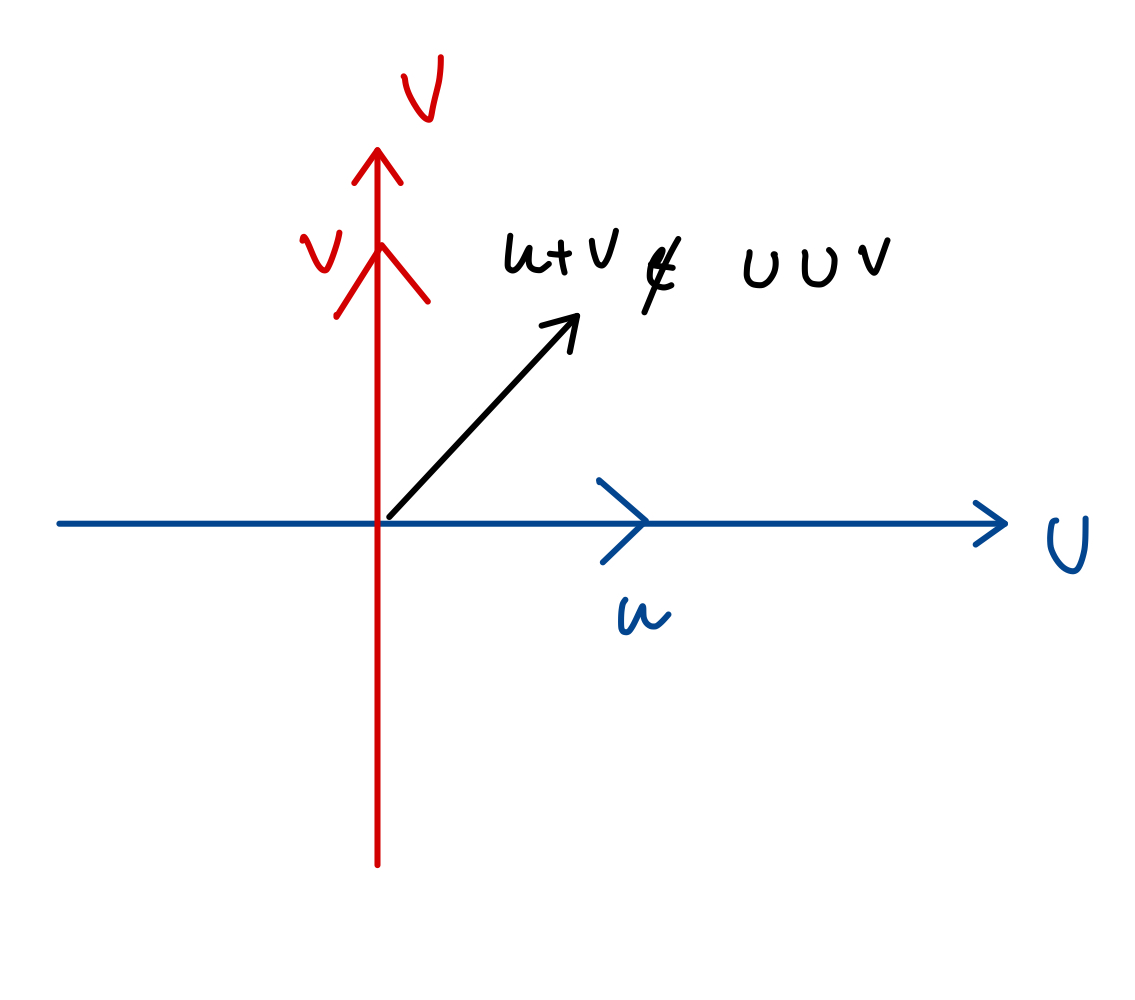
\includegraphics[scale=0.13]{la1.jpeg}
\end{center}

\begin{definition}[Sum of vector spaces]
    Let $V$ be a vector space over $\bbF$ and let $U,W\le V$. The \textit{sum} of $U,W$ is defined as 
    \[
        U+W  =\left\{ \bfu+\bfw: (\bfu,\bfw)\in U\times W \right\}.
    \] 
\end{definition}
For example, the sum of $x$-axis and $y$-axis is $ \mathbb{R}^{2} $. By direct verification we get:

\begin{proposition}
    $U+W\le V$.
\end{proposition}
\begin{proposition}
    $U+W$ is the smallest subspace of $V$ that contains $U,W$.
\end{proposition}
\begin{proof}
    Let $X$ be a subspace of $V$ that contains $U,W$. By closure, $ \bfu+\bfw\in X $ for all $ \bfu\in U,\bfw\in W $, so $ U+W\le X $. Hence it is the smallest subspace.
\end{proof}
\subsection{Subspaces and quotient}
Same as group theory, we can define subspaces and quotients. 
\begin{definition}[Quotient]
    Let $V$ a vector space over $\bbF$, and let $U \leq V$. The \emph{quotient space} $V/U$ is the abelian group $V/U$ equipped with the scalar multiplication $\bbF \times V/U \rightarrow V/U$, $(\lambda, \bfv + U) \mapsto \lambda \bfv + U$.
\end{definition}
The multiplication is well-defined, since if $ \bfv_1+U=\bfv_2+U $ then $ \bfv_1-\bfv_2\in U $, which implies $ \lambda(\bfv_1-\bfv_2) \in U$, and thus $ \lambda\bfv_1+U=\lambda\bfv_2+U\in V/U $.
\begin{proposition}
    $V/U$ is a vector space over $\bbF$.
\end{proposition}
\begin{proof}
    Let $ \lambda_1,\lambda_2\in \bbF $ and let $ \bfv_1+U,\bfv_2+U\in V/U $. Note that 
    \begin{align*}
        \lambda_1(\bfv_1+U)+\lambda_2(\bfv_2+U) &= (\lambda_1\bfv_1+U)+(\lambda_2\bfv_2+U)\\ 
        &= \lambda_1\bfv_1+\lambda_2\bfv_2+U\in V/U.\qedhere
    \end{align*}
\end{proof}

\subsection{Spans, independence and Steinitz Exchange Lemma}
\begin{definition}[Span of a Family of Vectors]
    Let $V$ be a vector space over $\mathbb F$ and $S\subset V$.
    We define the span of $S$ to be
    $$\langle S\rangle=\operatorname{span}(S)=\left\{\sum_{i=1}^n\lambda_i\bfs_i:n\in\mathbb N,\lambda_i\in \mathbb F,\bfs_i\in S\right\}$$
\end{definition}
That is, $\langle S\rangle$ consists of all possible \textit{finite} linear combination of elements of $S$.
By convention, $\langle \varnothing\rangle=\{0\}$.
\begin{remark}
    $ \langle S \rangle  $ is the smallest vector subspace of $V$ which contains $S$.
\end{remark}
\begin{example}
    \begin{enumerate}
        \item $V=\mathbb{R}^{3}$,
        \[
            S = \left\{\begin{pmatrix}
                1 \\ 0 \\ 0
            \end{pmatrix}, \begin{pmatrix}
                0 \\ 1 \\ 2
            \end{pmatrix}, \begin{pmatrix}
                3 \\ -2 \\ -4
            \end{pmatrix}\right\}.
        \]
        Verify that 
        \[
            \langle S \rangle = \left\{ \begin{pmatrix}
                a \\ b \\ 2b
            \end{pmatrix}:(a,b)\in \mathbb{R} \right\}.
        \]
        \item $ V = \mathbb{R}^{n} $, $\bfe_i$ standard basis, then $ V = \langle (\bfe_i)_{1\le i\le n} \rangle  $.
        \item Let $V=\mathbb R^X$ and $\delta_x:X\to\mathbb R$ be such that $\delta_x(y)=1_{x=y}$.
        Then $\langle \{\delta_x\}_{x\in\mathbb R}\rangle$ are the set of functions $f\in\mathbb R^X$ that has finite support ($ \operatorname{Supp} f = \{x:f(x)\neq 0\} $).
    \end{enumerate}
\end{example}
\begin{definition}
    Let $V$ be a vector space over $\mathbb F$ and $S\subset V$.
    We say $S$ spans $V$ if $\langle S\rangle =V$.
\end{definition}
\begin{example}
    Take $V=\mathbb R^2$, then any set of two non-parallel vectors would span $V$.
\end{example}
\begin{definition}
    A vector space $V$ over $\mathbb F$ is finite dimensional if there is a finite $S\subset V$ that spans $V$.
\end{definition}
\begin{example}
    $V=\mathbb P[x]$, the set of polynomials in $\mathbb R$ and $V_n=\mathbb P_n[x]$, the set of real polynomials with degree $\le n$.
    Then $V_n=\langle\{1,x,\ldots,x^n\}\rangle$ is finite dimensional, but $V$ is not finite dimensional as any finite set of polynomials must be contained in $V_n$ where $n$ is the maximal degree of polynomials in that set.
\end{example}
If $V$ is finite-dimensional, is there a minimal number of vectors in the family required so that the family spans $V$?
\begin{definition}[(Linear) Independence]
    Let $V$ be a vector space over $F$.

    We say $\{\bfv_1,\ldots,\bfv_n\}\subset V$ are (linearly) independent (or is a free family) if for any $\lambda_1,\ldots,\lambda_n\in F$
    $$\sum_{i=1}^n\lambda_i\bfv_i=0\implies\forall i,\lambda_i=0$$
    Equivalently, this set is not linearly independent if there exists $\lambda_1,\ldots,\lambda_n\in F$ not all zero such that $\sum_{i=1}^n\lambda_i\bfv_i=0$.
\end{definition}
\begin{example}
Let $V=\mathbb R^3$ and
$$\bfv_1=(1,0,0)^\top,\bfv_2=(0,1,0)^\top,\bfv_3=(1,1,0)^\top,\bfv_4=(0,1,1)^\top$$
Then $\{\bfv_1,\bfv_2\}$ is linearly independent.
Note that $\bfv_3\in\langle\{\bfv_1,\bfv_2\}\rangle$, so $\{\bfv_1,\bfv_2,\bfv_3\}$ is not linearly independent.
On the other hand, $\bfv_4\notin\langle\{\bfv_1,\bfv_2\}\rangle$, which as one can verify means that $\{\bfv_1,\bfv_2,\bfv_4\}$ is linearly independent.
\end{example}
\begin{remark}
    If the family $\{\bfv_i\}_{1\le i\le n}$ is linearly independent, then none of $\bfv_i$ is zero.
\end{remark}
\begin{definition}[Basis]
    A subset $S\subset V$ is a basis if it is linearly independent and $\langle S\rangle=V$.
\end{definition}
\begin{remark}
    When $S$ spans $V$, we say that $S$ is a generating family of $V$.
    So a basis is just a linearly independent(we also say free) generating family.
\end{remark}
\begin{example}
    \begin{enumerate}
        \item Take $V=\mathbb R^n$, then the family $\{\bfe_i\}_{1\le i\le n}$ where $\bfe_i$ is the vector having $1$ at $i^{th}$ entry and zero otherwise is a basis. $ (\bfe_i) $ are called the \textit{canonical basis}.
        \item Take $V=\mathbb C$ over $\mathbb C$, then $\{a\}$ is a basis for any $a\neq 0$.
        \item Take also $V=\mathbb C$ but over $\mathbb R$, then $\{1,i\}$ is a basis.
        \item Take $V=\mathbb P[x]$ be the set of polynomials in $\mathbb R$ and $S=\{x^n:n\ge 0\}$.
        Then $S$ is a basis.
        Worth noting that $|S|=\infty$ in this case.
    \end{enumerate}
\end{example}
\begin{lemma}
    If $V$ is a vector space over $F$, then $\{\bfv_1,\ldots,\bfv_n\}$ is a basis of $V$ if and only if for any vector $\bfv\in V$, there is a unique decomposition
    $$\bfv=\sum_{i=1}^n\lambda_i\bfv_i,\quad \lambda_i\in \mathbb{F}.$$
\end{lemma}
\begin{remark}
    If the conditions are true, then the tuple $(\lambda_1,\ldots,\lambda_n)$ (ordered via the ordering one chose on $\bfv_i$) is called the coordinate of $\bfv$ in the basis $(\bfv_i)$.
\end{remark}
\begin{proof}
    Suppose $ (\bfv_i) $ is a basis of $V$. This implies that $ \langle \bfv_i \rangle =V $, i.e. 
    \[
        \forall \bfv\in V\quad \exists (\lambda_1,\dots,\lambda_n)\in \bbF,\quad \bfv = \sum_{i=1}^{n}\lambda_i\bfv_i.
    \]
    Suppose that $ \exists (\lambda_i') $ s.t. the above holds, then 
    \[
        \sum_{i=n}^{n} \lambda_i-\lambda'_i=0 \Longrightarrow \lambda_i=\lambda_i'
    \]
    by independence.

    Suppose now that there is a unique decomposition. Then clearly $ \langle (\bfv_i) \rangle =V $. Consider 
    \[
        \sum_{i=1}^n\lambda_i\bfv_i=0,\quad \lambda_i\in \mathbb{F}.
    \]
    Clearly it is true for $ \lambda_i=0,\forall i $. By uniqueness, this is the only decomposition and thus $ (\bfv_i) $ is a basis.
\end{proof}
\begin{lemma}
    If $S$ is a finite set that spans $V$, then a subset of $S$ is a basis of $V$.
\end{lemma}
\begin{proof}
    If $S$ is independent, then we are done.
    Otherwise, there is some $\lambda\neq 0$ and $\lambda_\bfw$ such that there is $v\in S$ with
    $$\lambda \bfv+\sum_{\bfw\in S\setminus\{\bfv\}}\lambda_\bfw\bfw=0\implies \bfv=\frac{1}{\lambda}\sum_{\bfw\in S\setminus\{\bfv\}}\lambda_\bfw\bfw\in\langle S\setminus\{\bfv\}\rangle.$$
    Therefore $S\setminus\{\bfv\}$ also spans $V$.
    We can repeat this process and, by the well-ordering of $\mathbb N$, will reach a basis.
\end{proof}
\begin{theorem}[Steinitz Exchange Lemma]\label{thm:steinitz}
    Let $V$ be a finite dimensional vector space over $\bbF$. Take $\{\bfv_1,\ldots,\bfv_m\}\subset V$ linearly independent, $\{\bfw_1,\ldots,\bfw_n\}\subset V$ a generating set, then:
    \begin{enumerate}
        \item $m\le n$.
        \item Up to relabeling, $\{\bfv_1,\ldots,\bfv_m,\bfw_{m+1},\ldots,\bfw_n\}$ spans $V$.
    \end{enumerate}
\end{theorem}
\begin{proof}
    Suppose $\{\bfv_1,\ldots,\bfv_l,\bfw_{l+1},\ldots,\bfw_n\}$ spans $V$ for some $l<m$, then
    $$\exists\alpha_i,\beta_i\in \bbF, \bfv_{l+1}=\sum_{i\le l}\alpha_i\bfv_i+\sum_{i>l}\beta_i\bfw_i$$
    But $\{\bfv_i\}$ is linearly independent, so one of the $\beta_i$ is nonzero.
    By relabelling $\beta_{l+1}\neq 0$, then $\bfw_{l+1}\in\langle\{\bfv_1,\ldots,\bfv_l,\bfv_{l+1},\bfw_{l+2}\ldots,\bfw_n\}\rangle$, therefore the set of vectors 
    \[
        \{\bfv_1,\ldots,\bfv_l,\bfv_{l+1},\bfw_{l+2}\ldots,\bfw_n\}
    \]
    also spans $V$. If we start from 0, we are done after $m$ steps by induction, and thus $m\le n$, and
    \[
        \langle \bfv_1,\ldots,\bfv_m,\bfw_{m+1},\ldots,\bfw_n \rangle =V.\qedhere
    \]
\end{proof}

\subsection{Basis, Dimension and Direct Sum}
From the Steinitz Exchange Lemma, we have
\begin{corollary}\label{dim_well_defined}
    Let $V$ be a finite dimensional vector space, then any two bases of $V$ have the same cardinality.
\end{corollary}
We call this cardinality the \textit{dimension} of $V$, denoted by $ \dim V $ or $ \dim_\bbF V $, to specify the field.
\begin{corollary}
    Let $V$ be a vector space with $\dim V=n$, then:
    \begin{enumerate}
        \item Any independent set of vectors has size at most $n$.
        The size is exactly $n$ iff this set is a basis.
        \item Any spanning set has size at least $n$.
        The size is exactly $n$ iff this set is a basis.
    \end{enumerate}
\end{corollary}
\begin{proposition}
    Let $U,W$ be subspaces of $V$.
    If they are finite dimensional, then so is $U+W$ and
    $$\dim(U+W)=\dim U+\dim V-\dim(U\cap W)$$
\end{proposition}
\begin{proof}
    Pick a basis $\bfv_1,\ldots,\bfv_l$ of $U\cap W$ and extend it to a basis $\bfv_1,\ldots,\bfv_l,\bfu_1,\ldots,\bfu_m$ of $U$ and a basis $\bfv_1,\ldots,\bfv_l,$ $\bfw_1,\ldots,\bfw_n$ of $W$. 
    
    Claim that $B=\{\bfv_i\}\cup\{\bfu_i\}\cup\{\bfw_i\}$ is easily a basis of $U+W$.
    The equality follows.

    Indeed, it is obvious that $B$ is a generating set. To show linear independence, consider 
    \[
        \sum_{i=1}^{l}\alpha_i \bfv_i+\sum_{j=1}^{m}\beta_j \bfu_j+\sum_{k=1}^{n}\gamma_k\bfw_k=0.
    \]
    Rearrange this to get 
    \[
        \begin{aligned}
           & \sum_{i=1}^{l}\alpha_i \bfv_i+\sum_{j=1}^{m}\beta_j \bfu_j=-\sum_{k=1}^{n}\gamma_k\bfw_k\\ &\Longrightarrow \sum_{k=1}^{n}\gamma_k\bfw_k\in U \cap W\\ &\Longrightarrow \sum_{k=1}^{n}\gamma_k\bfw_k=\sum_{i=1}^{l}\delta_i\bfv_i.
        \end{aligned}
    \]
    Therefore we get 
    \[
        \sum_{i=1}^{l}(\alpha_i+\delta_i)\bfv_i+\sum_{j=1}^{m}\beta_j \bfu_j=0 \Longrightarrow \beta_j=0,\alpha_i=-\delta_i.
    \]
    Hence the original equation becomes 
    \[
        \sum_{i=1}^{l}\alpha_i\bfv_i+\sum_{k=1}^{n}\gamma_k\bfw_k=0 \Longrightarrow \alpha_i=\gamma_k=0.\qedhere
    \]
\end{proof}
\begin{proposition}
    If $V$ is a finite dimensional vectyor space and $U\le V$, then $U,V/U$ are both finite dimensional and $\dim V=\dim U+\dim V/U$.
\end{proposition}
\begin{proof}
    It is obvious that $U$ is finite dimensional.
    Choose a basis $\bfu_1,\ldots,\bfu_l$ and extend it to a basis $B=\{\bfu_1,\ldots,\bfu_l,\bfw_{l+1},\ldots,\bfw_n\}$ of $V$. Claim that $B'=\{\bfw_{l+1}+U,\ldots,\bfw_n+U\}$ is a basis of $V/U$ and we are done.

    Indeed, every non-trivial element in $ V/U $ has the form $ \bfv+U $, where $ \bfv\in V \setminus U $. Since $B$ is a basis, there exists $ \alpha_i,l+1\le i\le n $ such that 
    \[
        \bfv = \sum_{i=l+1}^{n}\alpha_i\bfw_i.
    \]
    Hence $ \bfv+U = \sum_{i=l+1}^{n}\alpha_i(\bfw_i +U)$ and thus $ B' $ generates $V/U$. To show independence, note that 
    \[
        \sum_{i=l+1}^{n}\beta_i \bfw_i+U=0 \Longrightarrow \sum_{i=l+1}^{n}\beta_i \bfw_i\in U \Longrightarrow \beta_i=0.\qedhere
    \]
\end{proof}
\begin{remark}
    If $U$ is a proper subspace of $V$, written $U<V$ (meaning that $U\le V$ and $U\neq V$), then the proposition gives us $\dim V/U\neq \{0\}$, so $\dim U<\dim V$.
\end{remark}
\begin{definition}
    Let $V$ be a vector space and $U,W\le V$.
    We say $V$ is the \textit{direct sum} of $U,W$, written $V=U\oplus W$, if every element $\bfv\in V$ can be written uniquely as $\bfv=\bfu+\bfw$ for $\bfu\in U,\bfw\in W$.
    If this happens, then we say $W$ is \textit{a direct complement} of $U$ in $V$.
\end{definition}
Note that direct complement is not unique in general.
\begin{example}
    Take $U=\mathbb R\times \{0\}$, then both $W=\{0\}\times \mathbb R$ and $W'=\langle\{(1,1)^\top\}\rangle$ are direct complements of $U$.
\end{example}
\begin{lemma}\label{equivalence_of_direct_sum}
    Let $U,W\le V$, then the followings are equivalent:
    \begin{enumerate}[(i)]
        \item $V=U\oplus W$.
        \item $V=U+W$ and $U\cap W=\{0\}$.
        \item For any basis $B_1$ of $U$ and $B_2$ of $W$, $B=B_1\cup B_2$ is a basis of $V$.
    \end{enumerate}
\end{lemma}
\begin{proof}
    (ii) $\Rightarrow$ (i): Suppose $V=U+W$ and $U\cap W=\{0\}$. Then $ \forall \bfv\in V,\exists (\bfu,\bfw)\in U\times W,\bfv=\bfu+\bfw $. To show uniqueness, suppose $ \bfv=\bfu_1+\bfw_1=\bfu_2+\bfw_2 $. Then $ \bfu_1-\bfu_2=\bfw_1-\bfw_2\in U \cap W=\{0\} $, so $ \bfu_1=\bfu_2,\bfw_1=\bfw_2$.

    (i) $\Rightarrow$ (iii): Let $ B_1,B_2 $ be bases of $U,W$ respectively. Let $ B=B_1 \cup B_2 $. Clearly $ \langle B \rangle =V $. Consider 
    \[
        \sum_{\bfu\in B_1}\lambda_{\bfu}\bfu+\sum_{\bfw\in B_2}\lambda_{\bfw}\bfw=0.
    \]
    Note that $ \lambda_\bfu=\lambda_\bfw=0 $ is a solution. Since $ V =U\oplus W $, the decomposition is unique so it is the only one, and we have independence.

    (iii) $\Rightarrow$ (ii): Any $\bfv\in V$ can be written as 
    \[
        \bfv=\sum_{\bfu\in B_1}\lambda_{\bfu}\bfu+\sum_{\bfw\in B_2}\lambda_{\bfw}\bfw
    \]
    so $ V=U+W $. Now let $ \bfv\in U\cap W $, then the above equation implies $\lambda_\bfu=\lambda_\bfw=0 $ and thus $ U\cap W=\{0\} $.
\end{proof}
\begin{definition}
    Let $V_1,\ldots,V_l\le V$, then we define
    $$\sum_{i=1}^lV_i=\{\bfv_1+\cdots+\bfv_l:\bfv_j\in V_j,1\le j\le l\}$$
    The sum is direct, i.e.
    $$\sum_{i=1}^lV_i=\bigoplus_{i=1}^lV_i$$
    if and only if $\bfv_1+\cdots +\bfv_l=\bfv_1'+\cdots +\bfv_l'$ implies $\bfv_j=\bfv_j'$ for any $1\le j\le l,\bfv_j\in V_j$ and $ \bfv_j'\in V_j $.
    Equivalently,
    $$V=\bigoplus_{i=1}^lV_i\iff \forall \bfv\in V,\exists!(\bfv_1,\ldots,\bfv_l)\in V_1\times\cdots\times V_l,\bfv=\sum_{i=1}^l\bfv_i.$$
\end{definition}
Lemma \ref{equivalence_of_direct_sum} is then generalized to
\begin{proposition}
    The followings are equivalent:
    \begin{enumerate}
        \item $\sum_{i=1}^lV_i=\bigoplus_{i=1}^lV_i$
        \item For any $i$,
        $V_i\cap\left( \sum_{j\neq i}V_j \right)=\{0\}$
        \item For any bases $B_i$ of $V_i$, the union $\bigcup_iB_i$ is a basis of $\sum_iV_i$.
    \end{enumerate}
\end{proposition}

\section{Linear Maps}
\subsection{Linear maps}
\begin{definition}[Linear Map]
    Let $V,W$ are vector spaces over $\bbF$, a function $\alpha:V\to W$ is \textit{linear} if for any $\lambda_1,\lambda_2\in \bbF$ and $\bfv_1,\bfv_2\in V$,
    $$\alpha(\lambda_1\bfv_1+\lambda_2\bfv_2)=\lambda_1\alpha(\bfv_1)+\lambda_2\alpha(\bfv_2).$$
\end{definition}
\begin{example}
    \begin{enumerate}
        \item Let $M$ be an $m\times n$ matrix, then $\alpha:\mathbb R^n\to\mathbb R^m$ via $x\mapsto Mx$ is a linear map.
        \item The functional $\alpha:C([0,1])\to C([0,1])$ via
        $$\alpha[f](x)=\int_0^xf(t)\,\mathrm dt$$
        is a linear map.
        \item Fix $x\in[a,b]$, then the evaluation map $\alpha:C([a,b])\to\mathbb R$ via $f\mapsto f(x)$ is a linear map.
    \end{enumerate}
\end{example}
\begin{remark}
    The identity map is a linear map.
    Composition of linear maps is also a linear map.
\end{remark}
\begin{lemma}
    Let $V,W$ be vector spaces over $\bbF$ and $B$ a basis for $V$.
    Let $\alpha_0:B\to W$ be a function, then there is a unique linear map $\alpha:V\to W$ that extends $\alpha_0$. i.e. $\exists \text{ linear }\alpha, \forall\bfv\in B, \alpha_0(\bfv)=\alpha(\bfv) $.
\end{lemma}
\begin{proof}
    For any $(\bfb_i)\in B$, necessarily $\alpha\left(\sum_i\lambda_i\bfb_i\right)=\sum_i\lambda\alpha_0(\bfb_i)$.
    This is sufficient.
\end{proof}
\begin{remark}
    This lemma is true for infinite dimensional vector spaces as well.
    Often, to define linear map, we often just define its values on a basis and extend it by this lemma.
\end{remark}
\begin{corollary}
    Two linear maps that agree on a basis are the same.
\end{corollary}
\subsection{Isomorphisms and the Rank-Nullity Theorem}
\begin{definition}
    Let $V,W$ be vector spaces over $\bbF$.
    A linear bijection $\alpha:V\to W$ is an \textit{isomorphism} (of vector spaces).
    If such a map exists, then we say $V,W$ are isomorphic (as vector spaces), written as $V\cong W$.
\end{definition}
\begin{remark}
    If $\alpha$ is an isomorphism, so is $\alpha^{-1}$.
\end{remark}
\begin{lemma}
    $\cong$ is an equivalence relation on the class of all vector spaces over $\bbF$.
\end{lemma}
\begin{proof}
    $i:V\to V$ is an isomorphism so $ V \cong V $. If $ \alpha:V\to W $ is an isomorphism then so is $ \alpha^{-1} $, and hence $ V \cong W \Rightarrow W \cong V $. If $ \beta:U\to V,\alpha:V\to W $ are isomorphisms, then $ \beta\circ \alpha:U\to W $ is an isomorphism and thus $ U \cong V \land V \cong W \Rightarrow U \cong W $. Hence it is an equivalence relation.
\end{proof}
\begin{theorem}
    If $V$ is a vector space over $\bbF$ of dimension $n$, then $V\cong \bbF^n$.
\end{theorem}
\begin{proof}
    Take a basis $\{\bfb_1,\ldots,\bfb_n\}$ of $V$, then $ \alpha:V\to \bbF^n $, defined by
    $$\alpha(x_1\bfb_1+\cdots+x_n\bfb_n)=(x_1,\ldots,x_n)^\top$$
    is an isomorphism.
\end{proof}
\begin{remark}
    Choosing a basis of $V$ is then just equivalent to choosing an isomorphism from $V$ to $\bbF^n$.
\end{remark}
\begin{theorem}\label{isom iff same dim}
    Let $V,W$ be finite dimensional vector spaces over $\bbF$.
    Then $V\cong W$ iff $\dim V=\dim W$.
\end{theorem}
\begin{proof}
    Any basis of $V$ induces a basis of $W$ via the isomorphism, so they have the same dimension.
    Therefore are both isomorphic to $\bbF^n$ where $n=\dim V=\dim W$.
\end{proof}
\begin{definition}
    Let $\alpha:V\to W$ be a linear map.
    We define the kernel of $\alpha$ to be $\ker\alpha=\{\bfv\in V:\alpha(\bfv)=0\}$ and the image to be $\operatorname{Im}\alpha=\alpha(V)=\{\bfw\in W:\exists \bfv\in V,\alpha(\bfv)=\bfw\}$.
\end{definition}
\begin{lemma}
    $\ker\alpha\le V,\operatorname{Im}\alpha\le W$.
\end{lemma}
\begin{example}
    Take $\alpha:C^\infty(\mathbb R)\to C^\infty(\mathbb R)$ by $\alpha(f)(t)=f^{\prime\prime}(t)+f(t)$.
    Then $\ker\alpha$ is spanned by $t\mapsto e^t$ and $t\mapsto e^{-t}$ and $\operatorname{Im}\alpha=C^{\infty}(\mathbb R)$.
\end{example}
There is a similar result to first isomorphism theorem:
\begin{theorem}
    Let $V,W$ be vector spaces over $F$ and $\alpha:V\to W$ be linear, then $V/{\ker\alpha}\cong \operatorname{Im}(\alpha)$ via $\bfv+\ker\alpha\mapsto \alpha(\bfv)$.
\end{theorem}
\begin{proof}
    Let $ \bar{\alpha} $ be the desired isomorphism(to be proved).

    Firstly check that $ \bar{\alpha} $ is well-defined. Indeed, if $ \bfv+\ker \alpha=\bfv'+\ker \alpha $, then $ \bfv-\bfv'\in \ker \alpha $ and thus $ \alpha(\bfv)=\alpha(\bfv')=0 $.

    Next show that $ \bar{\alpha} $ is a bijection. Let $ \bar{\alpha}(\bfv+\ker \alpha)=0 $, then $ \alpha(\bfv)=0 \Rightarrow \bfv+\ker \alpha=0+\ker \alpha $, so it is injective. Given $ \bfw\in \Im \alpha, \exists \bfv\in V $ such that $ \alpha(\bfv)=\bfw =\bar{\alpha}(\bfv+\ker \alpha)$, so it is surjective and hence bijective.
\end{proof}
\begin{definition}
    The rank of $\alpha:V\to W$ is $\rank(\alpha)=\dim\operatorname{Im}\alpha$ and nullity is $\nullity(\alpha)=\dim\ker\alpha$. Sometimes we write $ r(\alpha),n(\alpha) $. 
\end{definition}
Hence in the finite dimensional case, we can rewrite the preceding theorem to get
\begin{theorem}[Rank-Nullity Theorem]
    Let $\alpha:V\to W$ be linear where $V$ is finite dimensional.
    Then $\dim V=\rank(\alpha)+\nullity(\alpha)$.
\end{theorem}
\begin{proof}
    Since $ V/{\ker\alpha}\cong \operatorname{Im}(\alpha) $, we have 
    \begin{align*}
        & \dim (U/\ker \alpha)=\dim (\Im \alpha)\\ 
        \implies & \dim U-\dim \ker \alpha=\dim \Im \alpha\\ 
        \implies & \dim U = \rank \alpha+ \nullity \alpha.\qedhere
    \end{align*}
\end{proof}
\begin{corollary}[Classification of Isomorphism]
    Let $V,W$ be finite dimensional vector spaces with $\dim V=\dim W$ and $\alpha:V\to W$ be linear, then the followings are equivalent:
    \begin{enumerate}[(i)]
        \item $\alpha$ is injective.
        \item $\alpha$ is surjective.
        \item $\alpha$ is an isomorphism.
    \end{enumerate}
\end{corollary}
\begin{example}
    Consider
    $$V=\left\{ \begin{pmatrix}
        x\\
        y\\
        z
    \end{pmatrix}\in\mathbb R^3:x+y+z=0\right\}$$
    We want to compute $\dim V$.
    Consider $\alpha:\mathbb R^3\to\mathbb R$ via $(x,y,z)^\top\mapsto x+y+z$, then $r(\alpha)=1$ and $n(\alpha)=V$, so $\dim V=3-1=2$.
    Geometrically, $V$ is just a plane with normal $(1,1,1)^\top$.
\end{example}

\subsection{Linear Maps \texorpdfstring{$V \rightarrow W$}{V to W} and Matrices}
\subsubsection*{Space of linear maps}
We are now going to consider linear maps between two vector spaces $V$ and $W$.

\begin{definition}[Space of Linear Maps]
    Let $V$ and $W$ be vector spaces over $\bbF$. We define
    $$
    \mathcal{L}(V, W) = \{\alpha: V \rightarrow W \mid \alpha \text{ is a linear map}\}.
    $$
\end{definition}
\begin{proposition}
    $\mathcal{L}(V, W)$ is a vector space over $\bbF$.
    
    Moreover, if $V$ and $W$ are finite dimensional then so is $\mathcal{L}(V, W)$, and $\dim \mathcal{L}(V, W) = \dim V \cdot \dim W$.
\end{proposition}
\subsubsection*{Matrices}
\begin{definition}[Matrix]
    An $m \times n$ \emph{matrix} over $\bbF$ is an array with $m$ rows and $n$ columns, with entries in $\bbF$:
    $$
    A = (a_{ij}),
    $$
    with $1 \leq i \leq m$ and $1 \leq j \leq n$.

    The \textit{space of matrices} is the set $\mathcal{M}_{m,n}(\bbF)$ of $m \times n$ matrices over $\bbF$.
\end{definition}
By checking definitions we have
\begin{proposition}
    $ \mcM_{m,n}(\bbF) $ is a vector space over $ \bbF $.
\end{proposition}
\begin{proposition}
    $ \dim \mcM_{m,n}(\bbF) =m \times n$.
\end{proposition}
\begin{proof}
    We find an explicit basis. Pick $ 1\le i\le m,1\le j\le n $, define the \textit{elementary matrices} as
    \[
        E_{ij}=1 \text{ for entry } ij \text{ and } 0 \text{ elsewhere}.
    \]
    The set $\{E_{i, j} \mid 1 \leq i \leq m, 1 \leq j \leq m\}$ is clearly spanning and is also clearly linearly independent, so it is a basis. Counting elements, we see that this set has size $m \times n$, as required.
\end{proof}
\subsubsection*{Representation of linear maps by matrices}
Let $V$, $W$ be vector spaces over $\bbF$, and let $\alpha: V \rightarrow W$ be a linear map. 

Let $B = \{\bfv_1, \dots, \bfv_n\}$ be a basis for $V$, and $C = \{\bfw_1, \dots, \bfw_m\}$ be a basis for $W$. Then if $\bfv \in V$, we can write
$$
\bfv = \sum_{j = 1}^n \lambda_j \bfv_j = \begin{pmatrix}
    \lambda_1 \\ \vdots \\ \lambda_n
\end{pmatrix} \in \bbF^n,
$$
which are the `coordinates of $\bfv$' with the respect to the basis $B$, which we will call $[\bfv]_B$.

Similarly, for $\bfw \in W$, we can let $[\bfw]_C$ be the `coordinates' of $\bfw$ in the basis $C$.

\begin{definition}[Matrix of $\alpha$ in the $B, C$ Basis]
    We define $[\alpha]_{B, C}$, the \emph{matrix of $\alpha$} with respect to $B$ and $C$ by
    $$
    [\alpha]_{B, C} = \begin{pmatrix}
        [\alpha(\bfv_1)]_C, [\alpha(\bfv_2)]_C, \cdots, [\alpha(\bfv_n)]_C
    \end{pmatrix} \in \mathcal{M}_{m, n}(\bbF).
    $$ 
\end{definition}
\begin{lemma}
    For all $\v \in V$, we have $[\alpha(\v)]_C = [\alpha]_{B,C}  [\v]_B$.
\end{lemma}
\begin{proof}
    Let $\v \in V$, and let $\v = \sum_{j = 1}^n \lambda_j \v_j$. Then
    $$
    \alpha(\v) = \sum_{j = 1}^n \lambda_j \alpha(\v_j) = \sum_{j = 1}^n \lambda_j \sum_{i = 1}^m a_{ij} \w_i = \sum_{i = 1}^m \left(\sum_{j = 1}^n a_{ij} \lambda_j\right) \w_i,
    $$
    as required.
\end{proof}
By checking definitions,
\begin{lemma}
    Let $\alpha: V \rightarrow W$ and $\beta: U \rightarrow W$ be linear maps. Then if $A$ is a basis of $U$, $B$ is a basis of $V$ and $C$ is a basis of $W$, then
    $$
    [\alpha \circ \beta]_{A, C} = [\alpha]_{B, C}  [\beta]_{A, B}.
    $$
\end{lemma}
\begin{proposition}
    If $V$ and $W$ are vector spaces over $\bbF$ such that $\dim V = n$ and $\dim W = m$, then $\mathcal{L}(V, W) \cong \mathcal{M}_{m, n}(\bbF)$.
\end{proposition}
\begin{proof}
    Fix a basis $B, C$ of $V$ and $W$ respectively.
    Then consider the linear map
    $
    \theta: \mathcal{L}(V, W) \rightarrow \mathcal{M}_{m, n}(\bbF)
    $ given by $\alpha \mapsto [\alpha]_{B, C}$.
    This map is clearly linear. Let $ A=(a_{ij}) $, then the linear map 
    \[
        \alpha: \bfv_j\to \sum_{i=1}^{m}a_{ij}\w_i
    \]
    on bases $B,C$. Then $ \theta(\alpha)=A $ so it is surjective. Since a linear map is uniquely determined by the action on basis, $ \theta $ is surjective and hence bijective. Thus $\theta$ is an isomorphism and $ \mcL(V,W) \cong \mcM_{m,n}(\bbF) $. 

    Alternatively, the proposition is direct by theorem \ref{isom iff same dim}.
\end{proof}
\begin{remark}
    If $B$ is a basis of $V$, $C$ a basis of $W$, and 
    \[
        \epsilon_B:\begin{aligned}
            V&\to \bbF^n\\ 
            \bfv&\to [\bfv]_B
        \end{aligned}\quad \epsilon_C:\begin{aligned}
            W&\to \bbF^m\\ 
            \w &\to [\w]_C
        \end{aligned}
    \]
    then the following diagram commute:
    \begin{center}
        $\begin{tikzcd}
            V & W \\
            {\mathbb{F}^n} & {\mathbb{F}^m}
            \arrow["\alpha", from=1-1, to=1-2]
            \arrow["{\epsilon_B}"', from=1-1, to=2-1]
            \arrow["{[\alpha]_{B,C}}"', from=2-1, to=2-2]
            \arrow["{\epsilon_C}", from=1-2, to=2-2]
        \end{tikzcd}$
    \end{center}
\end{remark}

\begin{example}
    Let $V$ and $W$ be finite dimensional vector spaces.
    Consider the linear map $\alpha: V \rightarrow W$, and suppose $Y \leq V$. Consider the image of $Y$ under $\alpha$, $Z=\alpha(Y) = \{ \w \in W \mid \w= \alpha(\bfy), \bfy \in Y\}$.

    Define the sets $B' = \{\v_1, \dots, \v_k\}$ and $B'' = \{\v_{k + 1}, \dots, \v_n\}$ such that the union of disjoint sets $B = B' \cup B''$ is a basis for $V$, and $B'$ is a basis of $Y$ (that is, we extend using Steinitz exchange lemma).
    
    Similarity we define $C' = \{\w_1, \dots, \w_\ell\}$ and $C'' = \{\w_{\ell + 1}, \dots, \w_m\}$ such that the union of disjoint sets $C = C' \cup C''$ is a basis for $W$ and $C'$ is a basis for $\alpha(Y)$.

    Then we have the matrix
    $$ 
    [\alpha]_{B, C} = \begin{pmatrix}
        \alpha(\v_1) & \cdots & \alpha(\v_k) & \alpha(\v_{k + 1}) & \cdots & \alpha(\v_n)
    \end{pmatrix},
    $$
    and this will look like the block matrix
    $$
    \begin{pmatrix}
        A & B \\
        0 & C \\
    \end{pmatrix}
    $$
    where $A$ is $k \times \ell$ such that $ A = [\alpha\restriction_Y]_{B',C'} $. 
    Also $ \alpha $ induces a well-defined map $ \bar{\alpha}:V/Y\to W/Z $ such that $ \v+Y\mapsto \alpha(\bfv)+Z $, with matrix given by $ [\bar{\alpha}]_{B'',C''}=C $.
\end{example}
\subsection{Change of basis}
Suppose we have two bases $ B = \qty{\bfv_1, \dots, \bfv_n}, B' = \qty{\bfv_1', \dots, \bfv_n'} $ of $ V $ and corresponding $ C, C' $ for $ W $.
If we have a linear map $ [\alpha]_{B,C} $, we are interested in finding the components of this linear map in another basis, that is,
\[
	[\alpha]_{B,C} \mapsto [\alpha]_{B',C'}
\]
\begin{definition}
	The \textbf{change of basis} matrix $ P $ from $ B' $ to $ B $ is
	\[
		P = \begin{pmatrix}
			[\bfv_1']_B & \cdots & [\bfv_n']_B
		\end{pmatrix}
	\]
	which is the identity map in $ B' $, written
	\[
		P = [I]_{B', B}
	\]
\end{definition}
\begin{lemma}
	For a vector $ v $,
	\[
		[\bfv]_B = P [\bfv]_{B'}
	\]
\end{lemma}
\begin{proof}
	We have
	\[
		[\alpha(\bfv)]_C = [\alpha]_{B,C} \cdot [\bfv]_C
	\]
	Since $ P = [I]_{B', B} $,
	\[
		[I(\bfv)]_B = [I]_{B', B} \cdot [\bfv]_{B'} \implies [\bfv]_B = P[\bfv]_{B'}
	\]
	as required.
\end{proof}
\begin{remark}
	$ P $ is an invertible $ n \times n $ square matrix.
	In particular,
	\[
		P^{-1} = [I]_{B,B'}
	\]
	Indeed,
	\[
		I_n = [I \cdot I]_{B,B} = [I]_{B',B} \cdot [I]_{B',B}
	\]
	where $ I_n $ is the $ n \times n $ identity matrix.
\end{remark}
\begin{proposition}
	If $ \alpha $ is a linear map from $ V $ to $ W $, and $ P = [I]_{B',B}, Q = [I]_{C',C} $, we have
	\[
		A' = [\alpha]_{B',C'} = [I]_{C,C'}[\alpha]_{B,C}[I]_{B,'B} = Q^{-1}AP
	\]
	where $ A = [\alpha]_{B,C}, A' = [\alpha]_{B',C'} $.
\end{proposition}
\begin{proof}
	\begin{align*}
		[\alpha(\bfv)]_C                     &= Q [\alpha(\bfv)]_{C'}= Q [\alpha]_{B',C'} [\bfv]_{B'} = QA [\mathbf{v}]_{B'} \\
		[\alpha(\bfv)]_C                     & = [\alpha]_{B,C} [\bfv]_B        = AP[\bfv]_{B'}                  \\
		\implies \forall \bfv,\ QA[\bfv]_{B'} & = AP[\bfv]_{B'}                  \\
		\implies QA                     & = AP \implies A'=Q^{-1}AP.\qedhere
	\end{align*}
\end{proof}

\begin{definition}
	Matrices $ A, A' $ are called \textbf{equivalent} if
	\[
		A' = Q^{-1}AP
	\]
	for some invertible matrices $ Q\in \mathcal{M}_{m \times m}, P\in \mathcal{M}_{n \times n} $.
\end{definition}
\begin{remark}
	This defines an equivalence relation on $ M_{m,n}(F) $.
	\begin{itemize}
		\item $ A = I_m^{-1} A I_n $;
		\item $ A' = Q^{-1} AP \implies A = Q A' P^{-1} $;
		\item $ A' = Q^{-1}AP, A'' = (Q')^{-1}A'P' \implies A'' = (QQ')^{-1}A(PP') $.
	\end{itemize}
\end{remark}
\begin{proposition}
	Let $ \alpha \colon V \to W $ be a linear map.
	Then there exists a basis $ B $ of $ V $ and a basis $ C $ of $ W $ such that
	\[
		[\alpha]_{B,C} = \begin{pmatrix}
			I_r & 0 \\
			0   & 0
		\end{pmatrix}
	\]
	so the components of the matrix are exactly the identity matrix of size $ r $ in the top-left corner, and zeroes everywhere else.
\end{proposition}
\begin{proof}
    Keep in mind that
    \begin{quotation}
        \textit{If you choose a basis, choose it wisely.}
    \end{quotation}
	Fix $ r \in \mathbb N $ such that $ \dim \ker \alpha = n - r $,
	and construct a basis $ \qty{\bfv_{r+1}, \dots, \bfv_n} $ of the kernel.
	Extend this to a basis of the entirety of $ V $, that is, $ \qty{\bfv_1,\dots,\bfv_n} $.
    We want to show that
	\[
		\qty{\alpha(\bfv_1), \dots, \alpha(\bfv_r)}
	\]
	is a basis of $ \Im \alpha $.

	Indeed, it spans $W$:
	\[
        \bfv         = \sum_{i=1}^n \lambda_i \bfv_i,         \quad
		\alpha(\bfv) = \sum_{i=1}^n \lambda_i \alpha(\bfv_i)
		          = \sum_{i=1}^r \lambda_i \alpha(\bfv_i)
    \]
	Then if $ \bfy \in \Im \alpha $, there exists $ \bfv $ such that $ \alpha(\bfv) = \bfy $, i.e. $ \mathbf{y} $ is in the span.

	Further, it is linearly independent:
	\begin{align*}
		\sum_{i=1}^r \lambda_i \alpha(\bfv_i) = 0&\implies
		\alpha\qty(\sum_{i=1}^r \lambda_i \bfv_i)= 0 \implies
		\sum_{i=1}^r \lambda_i \bfv_i \in \ker \alpha \\
        &\implies \sum_{i=1}^r \lambda_i \bfv_i = \sum_{i=r+1}^n \lambda_i \bfv_i \\
		&\implies \sum_{i=1}^r \lambda_i \bfv_i - \sum_{i=r+1}^n \lambda_i \bfv_i  = 0.
	\end{align*}
	But since $ \qty{\bfv_1, \dots, \bfv_n} $ is a basis, $ \lambda_i = 0 $ for all $ i $.
	Hence $ \qty{\alpha(\bfv_i)} $ is a basis of $ \Im \alpha $.

	Now, extend this basis to the whole of $ W $ to form
	\[
		\qty{\alpha(\bfv_1), \dots, \alpha(\bfv_r), \bfw_{r+1}, \dots, \bfw_n}
	\]
	Now,
	\begin{align*}
		[\alpha]_{BC} & = \begin{pmatrix}
			\alpha(\bfv_1) & \cdots & \alpha(\bfv_r) & \alpha(\bfv_{r+1}) & \cdots & \alpha(\bfv_n)
		\end{pmatrix} \\
		              & = \begin{pmatrix}
			I_r & 0 \\
			0   & 0
		\end{pmatrix}\qedhere
	\end{align*}
\end{proof}
\begin{remark}
	This also proves the rank-nullity theorem:
	\[
		\rank \alpha + \nullity \alpha = n
	\]
\end{remark}
\begin{corollary}
	Any $ m \times n $ matrix $ A $ is equivalent to a matrix of the form
	\[
		\begin{pmatrix}
			I_r & 0 \\
			0   & 0
		\end{pmatrix}
	\]
	where $ r = \rank A $.
\end{corollary}

\subsection{Rank of matrices}\ \vspace*{-1.5em}
\begin{definition}
	Let \( A \in M_{m,n}(\bbF) \).
	Then, the \textbf{column rank} of \( A \), \( r_c(A) \), is the dimension of the subspace of \( \mathbb{F}^n \) spaned by the column vectors.
	\[
		r_c(A) = \dim \operatorname{span} \qty{\bfc_1, \dots, \bfc_n}.
	\]

    Similarly, the \textbf{row rank} of $A$ is defined by $ r(A^\top) $.
\end{definition}

\begin{remark}
	If \( \alpha \) is a linear map, represented in bases \( B, C \) by the matrix \( A \), then
	\[
		\rank \alpha = r_c(A). 
	\]
    i.e. column rank $=$ rank.
\end{remark}

\begin{proposition}
	Two matrices are equivalent if and only if they have the same column rank:
	\[
		r_c(A) = r_c(A')
	\]
\end{proposition}
\begin{proof}
	If the matrices are equivalent, then \( A = [\alpha]_{BC}, A' = [\alpha]_{B',C'} \).
	Then
	\[
		r_c(A) = r_c(\alpha) = r_c(A')
	\]
	Conversely, if \( r_c(A) = r_c(A') = r \), then \( A, A' \) are equivalent to
	\[
		\begin{pmatrix}
			I_r & 0 \\
			0   & 0
		\end{pmatrix}
	\]
	which indicates \( A, A' \) are equivalent.
\end{proof}

\begin{theorem}
    $ r_c(A) = r_c(A^\top) $. 
\end{theorem}
\begin{proof}
    Let $ r = r_c(A) $. We know that $A$ is equivalent to the matrix 
    \[
        Q^{-1}AP = \begin{pmatrix}
			I_r & 0 \\
			0   & 0
		\end{pmatrix}_{m\times n}
    \]
    Take the transpose
    \[
		P^\top A^\top \qty(Q^{-1})^\top = (Q^{-1}AP)^\top = \begin{pmatrix}
			I_r & 0 \\
			0   & 0
		\end{pmatrix}_{m \times n}^\top = \begin{pmatrix}
			I_r & 0 \\
			0   & 0
		\end{pmatrix}_{n \times m}
	\]
    which proves the theorem. 
\end{proof}

Hence we can just write $ r(A) $, without subscript.

\subsection{Elementary operations and elementary matrices}
\paragraph{Aside: change of basis in the same space} Consider the following special case of changing basis.
If \( \alpha \colon V \to V \) is linear, \( \alpha \) is called an \textbf{endomorphism}.
If \( B = C, B' = C' \) then the special case of the change of basis formula is
\[
	[\alpha]_{B',B'} = P^{-1} [\alpha]_{B,B} P
\]
Then, we say square matrices \( A, A' \) are \textbf{similar} or \textbf{conjugate} if there exists \( P \) such that \( A' = P^{-1} A P \).

\begin{definition}
	An \textbf{elementary column operation} is
	\begin{enumerate}[(i)]
		\item swap columns \( i, j \)
		\item replace column \( i \) by \( \lambda \) multiplied by the column
		\item add \( \lambda \times\) column \( i \) to column \( j \ (i\neq j)\)
	\end{enumerate}
\end{definition}

\begin{note}
    \begin{itemize}
        \item Elementary row operations are defined similarly. 
        \item The elementary operations are invertible. 
    \end{itemize}
\end{note}

These operations can be described through the action of \textbf{elementary matrices}: 
\begin{definition}
    The elementary matrices are defined by 
    \begin{enumerate}[(i)]
        \item Swap columns $i,j$  
        \[
            T_{ij} = \begin{pmatrix}
                I_n & 0 & 0   \\
                0   & A & 0   \\
                0   & 0 & I_m
            \end{pmatrix};\quad A = \begin{pmatrix}
                0 & 0   & 1 \\
                0 & I_k & 0 \\
                1 & 0   & 1
            \end{pmatrix}
        \]
        \item Multiply column $i$ by $\lambda$  
        \[
            M_{i,\lambda} = \begin{pmatrix}
                I_n & 0       & 0   \\
                0   & \lambda & 0   \\
                0   & 0       & I_m
            \end{pmatrix}
        \]
        \item Add a multiple of a column,
        \[
            C_{ij,\lambda} = I + \lambda E_{ij},\quad E_{ij} \text{ is the standard basis}
        \]
    \end{enumerate}
\end{definition}

An elementary column (or row) operation can be performed by multiplying \( A \) by the corresponding elementary matrix from the right (on the left for row operations).

This provides a constructive proof that any \( n \times n \) matrix is equivalent to
\[
	\begin{pmatrix} I_r & 0 \\ 0 & 0 \end{pmatrix}
\]
\begin{proof}
    Start with $A$. If all entries are 0, we are done. 

    Pick $ a_{ij} = \lambda\neq 0 $: 
    \begin{itemize}
        \item Swap rows $i$ and $1$ 
        \item Swap columns $i$ and $1$ 
    \end{itemize}
    We get $ \lambda = a_{11} $, and by multiplying $ 1/\lambda $ we get $ a_{11}= 1 $. 

    Now the matrix becomes 
    \[
        \begin{pmatrix}
            1 &  0 \\
            0 &  \tilde{A} \\
        \end{pmatrix},\quad \tilde{A}\in \mathcal{M}_{(n-1),(n-1)} 
    \]
    and we can proceed inductively. After a finite step we get 
    \[
        \begin{pmatrix} I_r & 0 \\ 0 & 0 \end{pmatrix} = Q^{-1}AP = \underbrace{E'_\ell \cdots E'_1}_{\text{row operations}} A \underbrace{E_1 \cdots E_{l}}_{\text{column operations}}\qedhere
    \]
\end{proof}

\subsection{Gauss' pivot algorithm, finding inverses}

If we use only row operations, we can reduce each matrix to the so-called \textbf{row echelon form}: 
\[
    \begin{pmatrix}
        1 & 0 & \cdots & 0 &  b \\
        0 & \cdots & 1 & 0 &  c \\
        0 & \cdots & 0 & 1 &  d \\
    \end{pmatrix}
\]
where the `1's are pivots. The algorithm is described as follows 
\begin{enumerate}
    \item Assume $a_{i1}\neq 0$ for some $i$
    \item Swap rows $i$ and $1$ 
    \item Divide first row by $ \lambda = a_{i 1} $ to get $a_{11}=1$ 
    \item Use 1 to clear the rest of the first column
    \item Move to the second column and repeat
\end{enumerate}

This process is exactly the process used to solve a linear system of equations (Gaussian elimination).

\begin{lemma}
	If \( A \) is an \( n \times n \) square invertible matrix, then we can obtain \( I_n \) using only row elementary operations, or only column elementary operations.
\end{lemma}
\begin{proof}
	We show an algorithm that constructs this \( I_n \).
	This is exactly going to invert the matrix, since the resultant operations can be combined to get the inverse matrix.
	We will show here the proof for column operations.
	We argue by induction on the number of rows.
	Suppose we can make the form
	\[
		\begin{pmatrix} I_k & 0 \\ A & B \end{pmatrix}
	\]
	We want to obtain the same structure with \( k+1 \) rows.
	We claim that there exists \( j > k \) such that \( a_{k+1,j} \neq 0 \).
	Indeed, otherwise we can show that the vector
	\[
		\begin{pmatrix} 0 \\ \vdots \\ 1 \\ \vdots \\ 0 \end{pmatrix} = \delta_{k+1,i}
	\]
	is not in the span of the column vectors of \( A \).
	This contradicts the invertibility of the matrix.
	Now, we will swap columns \( k+1, j \) and divide this column by \( \lambda \).
	We can now use this 1 to clear the rest of the \( k+1 \) row.

	Inductively, we have found \( A E_1 \dots E_n = I_n \) where \( E_n \) are elementary.
	Thus, we can find \( A^{-1} \).
\end{proof}
\begin{proposition}
	Any invertible square matrix is a product of elementary matrices.
\end{proposition}
The proof is exactly the proof of the lemma above.


\section{Dual spaces and dual maps}
\subsection{Dual spaces}\ \vspace*{-1.5em}
\begin{definition}
	Let \( V \) be an \( \mathbb{F} \)-vector space.
	Then \( V^* \) is the \textbf{dual} of \( V \), defined by
	\[
		V^* = L(V,\mathbb F) = \qty{\alpha \colon V \to \mathbb F}
	\]
	where the \( \alpha \) are linear.
	If \( \alpha \colon V \to \mathbb F \) is linear, then we say \( \alpha \) is a linear form.
	So the dual of \( V \) is the set of linear forms on \( V \).
\end{definition}
\begin{example}
	The trace \( \operatorname{tr} \colon M_{n,n}(\mathbb F) \to \mathbb F \) is a linear form on \( M_{n,n}(\mathbb F) \).
\end{example}
\begin{example}
	Consider functions \( [0,1] \to \mathbb R \).
	We can define \( T_f \colon C^\infty([0,1], \mathbb R) \to \mathbb R \) such that \( \phi \mapsto \int_0^1 f(x) \phi(x) \dd{x} \).
	Then \( T_f \) is a linear form on \( C^{\infty}([0,1], \mathbb R) \).
	We can then reconstruct \( f \) given \( T_f \).
	This mathematical formulation is called distribution.
\end{example}
\begin{lemma}
	Let \( V \) be an \( \mathbb F \)-vector space with a finite basis \( B = \qty{\bfe_1, \dots, \bfe_n} \).
	Then there exists a basis \( B^* \) for \( V^* \) given by
	\[
		B^* = \qty{\varepsilon_1, \dots, \varepsilon_n}; \quad \varepsilon_j \qty( \sum_{i=1}^n a_i \bfe_i ) = a_j
	\]
	We call \( B^* \) the \textbf{dual basis} for \( B \).
\end{lemma}
We know
\[
    \varepsilon_j \qty( \sum_{i=1}^n a_i \bfe_i ) = a_j
\]
Equivalently,
\[
    \varepsilon_j (\bfe_i) = \delta_{ij}
\]
\begin{proof}
	First, we will show that the set of linear forms as defined is linearly independent.
	For all \( i \),
	\[
        \sum_{j=1}^n \lambda_j \varepsilon_j= 0 \implies
		\qty( \sum_{j=1}^n \lambda_j \varepsilon_j ) \bfe_i = 0 \implies
		\sum_{j=1}^n \lambda_j \varepsilon_j(e_i)                   = 0 \implies
		\lambda_i = 0.
    \]
	Now we show that the set spans \( V^* \).
	Suppose \( \alpha \in V^* \), \( x \in V \).
	\[
        \alpha(x) = \alpha\qty(\sum_{j=1}^n \lambda_j \bfe_j)
		           = \sum_{i=1}^n \lambda_j \alpha(\bfe_j)
    \]
	Conversely, let
	\[
		\sum_{i=1}^n \alpha(\bfe_j) \varepsilon_j \in V^*
	\]
	Then
	\begin{align*}
		\qty( \sum_{i=1}^n \alpha(\bfe_j) \varepsilon_j) (\bfx) & = \sum_{j=1}^n \alpha(\bfe_j) \varepsilon_j\qty(\sum_{k=1}^n \lambda_k \bfe_k) \\
        & = \sum_{j=1}^n \alpha(\bfe_j) \sum_{k=1}^n \lambda_k \varepsilon_j(\bfe_k)     \\
        & = \sum_{j=1}^n \alpha(\bfe_j) \sum_{k=1}^n \lambda_k \delta_{jk}            \\
        & = \sum_{j=1}^n \alpha(\bfe_j) \lambda_j                                     \\
        & = \alpha(\bfx)
	\end{align*}
	We have then shown that
	\[
		\alpha = \sum_{j=1}^n \alpha(\bfe_j) \varepsilon_j
	\]
	as required.
\end{proof}
\begin{corollary}
	If \( V \) is finite-dimensional, then $ \dim V = \dim V^* $.
\end{corollary}
\begin{remark}
	It is sometimes convenient to think of \( V^* \) as the spaces of row vectors of length \( \dim V \) over \( \bbF \).
	For instance, consider the basis \( B = (\bfe_1, \dots, \bfe_n) \), so \( \bfx = \sum_{i=1}^n x_i \bfe_i \).
	Then we can pick \( (\varepsilon_1, \dots, \varepsilon_n) \) a basis of \( V^* \), so \( \alpha = \sum_{i=1}^n \alpha_i \varepsilon_i \).
	Then
	\[
		\alpha(\bfx) = \sum_{i=1}^n \alpha_i \varepsilon_i(\bfx) = \sum_{i=1}^n \alpha_i \varepsilon\qty(\sum_{j=1}^n x_j \bfe_j) = \sum_{i=1}^n \alpha_i x_i
	\]
	This is exactly
	\[
		\begin{pmatrix} \alpha_1 & \cdots & \alpha_n \end{pmatrix} \begin{pmatrix} x_1 \\ \vdots \\ x_n \end{pmatrix}
	\]
	which essentially defines a scalar product between the two spaces.
\end{remark}

\subsection{Annihilators}\ \vspace*{-1.5em}
\begin{definition}
	Let \( U \subseteq V \).
	Then the annihilator of \( U \) is
	\[
		U^0 = \qty{\alpha \in V^* \colon \forall \bfu \in U, \alpha(\bfu) = 0}
	\]
\end{definition}
\begin{lemma}
	\begin{enumerate}[(i)]
		\item \( U^0 \leq V^* \);
		\item If \( U \leq V \) and \( \dim V < \infty \), then \( \dim V = \dim U + \dim U^0 \).
	\end{enumerate}
\end{lemma}
\begin{proof}
	\begin{enumerate}[(i)]
		\item First, note that \( 0 \in U^0 \) since \( \alpha(0) = 0 \) by linearity.
		      If \( \alpha, \alpha' \in U^0 \), then for all \( \bfu \in U \),
		      \[
			      (\alpha + \alpha')(\bfu) = \alpha(\bfu) + \alpha'(\bfu) = 0
		      \]
		      Further, for all \( \lambda \in F \),
		      \[
			      (\lambda \alpha)(\bfu) = \lambda \alpha(\bfu) = 0
		      \]
		      Hence \( U^0 \leq V^* \).
		\item Let \( (\bfe_1, \dots, \bfe_k) \) be a basis of \( U \) and extend it to a basis
		\[
            B = (\bfe_1, \dots, \bfe_k, \bfe_{k+1}, \dots, \bfe_n)
        \]
		      Let \( (\varepsilon_1, \dots, \varepsilon_n) \) be the dual basis \( B^* \).
		      We then will prove that
		      \[
			      U^0 = \langle\varepsilon_{k+1}, \dots, \varepsilon_n\rangle
		      \]
		      If \( i > k \), then \( \varepsilon_i(e_k) = \delta_{ik} = 0 \).
		      Hence \( \varepsilon_i \in U^0 \).
		      Thus \( \langle{\varepsilon_{k+1}, \dots, \varepsilon_n}\rangle \subset U^0 \).
		      Let \( \alpha \in U^0 \).
		      Then \( \alpha = \sum_{i=1}^n \alpha_i \varepsilon_i \).
		      For \( i \leq k \), \( \alpha \in U^0 \) hence \( \alpha(e_i) = 0 \).
		      Hence,
		      \[
			      \alpha = \sum_{i=k+1}^n \alpha_i \varepsilon_i
		      \]
		      Thus
		      \[
			      \alpha \in \langle{\varepsilon_{k+1}, \dots, \varepsilon_n}\rangle
		      \]
		      as required.\qedhere
	\end{enumerate}
\end{proof}

\subsection{Dual maps}\ \vspace{-1.5em}
\begin{lemma}
	Let \( V, W \) be \( \bbF \)-vector spaces.
	Let \( \alpha \in L(V,W) \).
	Then there exists a unique \( \alpha^* \in L(W^*, V^*) \) such that
	\[
		\varepsilon \mapsto \varepsilon \circ \alpha
	\]
	It is called the \textbf{dual map}.
\end{lemma}
\begin{proof}
	\( \varepsilon(\alpha) \colon V \to \bbF \) linear by linearity of $ \varepsilon, \alpha $,	so \( \varepsilon \circ \alpha \in V^* \).
	Now we show \( \alpha^* \) is linear:
	\[
		\alpha^*(\theta_1 + \theta_2) = (\theta_1 + \theta_2)(\alpha) = \theta_1 \circ \alpha + \theta_2 \circ \alpha = \alpha^*(\theta_1) + \alpha^*(\theta_2)
	\]
	and
	\[
		\alpha^*(\lambda \theta) = \lambda \alpha^*(\theta)
	\]
	as required.
	Hence \( \alpha^* \in L(W^*, V^*) \).
\end{proof}
\begin{proposition}
	Let \( V, W \) be finite-dimensional \( \bbF \)-vector spaces with bases \( B, C \) respectively.
	Then
	\[
		[\alpha^*]_{C^*, B^*} = [\alpha]^\top_{B, C}
	\]
	Thus, we can think of the dual map as the \textit{adjoint} of \( \alpha \).
\end{proposition}
\begin{proof}
	Let \( B = (b_1, \dots, b_n) \), \( C = (c_1, \dots, c_m) \), \( B^* = (\beta_1, \dots, \beta_n) \), \( C^* = (\gamma_1, \dots, \gamma_m) \).
	Let \( [\alpha]_{B,C} = (a_{ij}) \).
	Then
	\begin{align*}
		\alpha^*(\gamma_r)(b_s) & = \gamma_r \circ \alpha(b_s)= \gamma_r \qty( \sum_t a_{ts} c_t ) \\
		                            & = \sum_t a_{ts} \gamma_r(c_t) = \sum_t a_{ts} \delta_{tr}          \\
		                            & = a_{rs}
	\end{align*}
	We can conversely write \( [\alpha^*]_{C^*, B^*} = (m_{ij}) \) and
	\begin{align*}
		\alpha^*(\gamma_r)      & = \sum_{i=1}^n m_{ir} \beta_i      \\
		\alpha^*(\gamma_r)(b_s) & = \sum_{i=1}^n m_{ir} \beta_i(b_s)= \sum_{i=1}^n m_{ir} \delta_{is}  \\
		                            & = m_{sr}
	\end{align*}
	which gives $ a_{rs} = m_{sr} $, as required.
\end{proof}

\subsection{Properties of the dual map, double dual}

Let \( \alpha \in L(V,W) \), and \( \alpha^* \in L(W^*, V^*) \).
Let \( B \) and \( C \) be bases of \( V, W \) respectively, and \( B^*, C^* \) be their duals.
We have proven that
\[
	[\alpha]_{B,C} = [\alpha^*]^\top_{B,C}
\]
\begin{lemma}
	Suppose that \( E = (e_1, \dots, e_n) \) and \( F = (f_1, \dots, f_n) \) are bases of \( V \).
	Let \( P = [I]_{F, E} \) be a change of basis matrix from \( F \) to \( E \).
	The bases \( E^* = (\varepsilon_1, \dots, \varepsilon_n) \), \( F^* = (\eta_1, \dots, \eta_n) \) are the corresponding dual bases.
	Then, the change of basis matrix from \( F^* \) to \( E^* \) is
	\[
		\qty(P^{-1})^\top
	\]
\end{lemma}
\begin{proof}
	Consider
	\[
		[I]_{F^*, E^*} = [I]^\top_{E, F} = \qty([I]_{F, E}^{-1})^\top = \qty(P^{-1})^\top
	\]
\end{proof}
\begin{lemma}
	Let \( V, W \) be \( \bbF \)-vector spaces.
	Let \( \alpha \in L(V, W) \).
	Let \( \alpha^* \) be the corresponding dual map.
	Then, denoting \( N(\alpha) \) for the kernel of \( \alpha \),
	\begin{enumerate}[(i)]
		\item \( N(\alpha^*) = (\Im \alpha)^0 \), so \( \alpha^* \) is injective if and only if \( \alpha \) is surjective.
		\item \( \Im \alpha^* \leq (N(\alpha))^0 \), with equality if \( V, W \) are finite-dimensional.
		      In this finite-dimensional case, \( \alpha^* \) is surjective if and only if \( \alpha \) is injective.
	\end{enumerate}
\end{lemma}
\begin{remark}
	In many applications, it is often simpler to understand the dual map \( \alpha^* \) than it is to understand \( \alpha \).
\end{remark}
\begin{proof}
	\begin{enumerate}[(i)]
        \item Let $ \epsilon\in W^* $. Then
        \begin{align*}
            \epsilon\in N(\alpha^*) &\iff \alpha^*(\epsilon) = 0 \iff \epsilon\circ \alpha = 0 \\ 
            &\iff \forall \mathbf{v}\in V, \ \epsilon(\alpha(\mathbf{v})) = 0\\ 
            &\iff \epsilon\in (\Im(\alpha))^0. 
        \end{align*}
        \item Let \( \varepsilon \in \Im \alpha^* \).
        Then \( \alpha^*(\phi) = \varepsilon \) for some \( \phi \in W^* \).
        Then, for all \( \bfu \in N(\alpha) \), \( \varepsilon(\bfu) = \qty(\alpha^*(\phi))(\bfu) = \phi \circ \alpha(\bfu) = \phi(\alpha(\bfu)) = 0 \).
        So \( \Im \alpha^* \leq (N(\alpha))^0 \).
    
        In the finite-dimensional case, we can compare the dimension of these two spaces.
        \begin{align*}
            \dim \Im \alpha^* &= r(\alpha^*) = r\qty([\alpha^*]_{C^*, B^*}) \\ 
            &= r\qty([\alpha]_{B,C}^\top) = r\qty([\alpha]_{B,C}) = r(\alpha) = \dim \Im \alpha
        \end{align*}
        Due to the rank-nullity theorem, \( \dim \Im \alpha^* = \dim V - \dim N(\alpha) = \dim\qty[(N(\alpha))^0] \).
        Hence,
        \[
            \Im \alpha^* \leq (N(\alpha))^0;\quad \dim \Im \alpha^* = \dim (N(\alpha))^0
        \]
        The dimensions are equal, and one is a subspace of the other, hence the spaces are equal.
    \end{enumerate}
\end{proof}

\begin{definition}
	Let \( V \) be an \( \bbF \)-vector space.
	Let \( V^* \) be the dual of \( V \).
	The \textbf{double dual} or \text{bidual} of \( V \) is
	\[
		V^{* *} = L(V^*, \bbF) = (V^*)^*
	\]
\end{definition}
\begin{remark}
	In general, there is no obvious relation between \( V \) and \( V^* \).
	However, the following useful facts hold about \( V \) and \( V^{* *} \).
	\begin{enumerate}
		\item There is a \textit{canonical embedding} from \( V \) to \( V^{* *} \).
		      In particular, there exists \( i \) in \( L(V, V^{* *}) \) which is injective.
		\item There are examples of infinite-dimensional spaces where \( V \simeq V^{* *} \).
		      These are called reflexive spaces.
		      Such spaces are investigated in the study of Banach spaces.
	\end{enumerate}
\end{remark}
\begin{theorem}
	\( V \) embeds into \( V^{* *} \).
\end{theorem}
\begin{proof}
	Choose a vector \( \bfv \in V \) and define the linear form \( \hat v \in L(V^*, F) \) such that
	\[
		\hat v(\varepsilon) = \varepsilon(\mathbf{v})
	\]
	So clearly \( \hat v \) is linear.
	We want to show \( \hat v \in V^{* *} \).
	If \( \varepsilon \in V^*, \varepsilon(v) \in F \).
	Further, \( \lambda_1, \lambda_2 \in F \) and \( \varepsilon_1, \varepsilon_2 \in V^* \) give
	\[
		\hat v (\lambda_1 \varepsilon_1 + \lambda_2 \varepsilon_2) = (\lambda_1 \varepsilon_1 + \lambda_2 \varepsilon_2)(v) = \lambda_1 \varepsilon_1(v) + \lambda_2 \varepsilon_2(v) = \lambda_1 \hat v(\varepsilon_1) + \lambda_2 \hat v(\varepsilon_2)
	\]
\end{proof}
\begin{theorem}
	If \( V \) is finite-dimensional, then \( i \colon V \to V^{* *} \) given by \( i(\bfv) = \hat v \) is an isomorphism.
\end{theorem}
\begin{proof}
	We will show \( i \) is linear.
	If \( \bfv_1, \bfv_2 \in V, \lambda_1, \lambda_2 \in F \), then
	\[
		i(\lambda_1 \bfv_1 + \lambda_2 \bfv_2) (\varepsilon) = \varepsilon(\lambda_1 \bfv_1 + \lambda_2 \bfv_2) = \lambda_1 \varepsilon(\bfv_1) + \lambda_2 \varepsilon(\bfv_2) = \lambda_1 \hat v_1(\varepsilon) + \lambda_2 \hat v_2(\varepsilon)
	\]
	Now, we will show that \( i \) is injective for finite-dimensional \( V \).
	Let \( \bfe \in V \setminus \qty{0} \).
	We will show that \( \bfe \not\in \ker i \)
    .
	We extend \( \bfe \) into a basis \( (\bfe, \bfe_2, \dots, \bfe_n) \) of \( V \).
	Now, let \( (\varepsilon, \varepsilon_2, \dots, \varepsilon_n) \) be the dual basis.
	Then \( \hat e(\varepsilon) = \varepsilon(\bfe) = 1 \).
	In particular, \( \hat e \neq 0 \).
	Hence \( \ker i = \qty{0} \), so it is injective.

	We now show that \( i \) is an isomorphism.
	We need to simply compute the dimension of the image under \( i \).
	Certainly, \( \dim V = \dim V^* = \dim (V^*)^* = \dim V^{* *} \).
	Since \( i \) is injective, \( \dim V = \dim V^{* *} \).
	So \( i \) is surjective as required.
\end{proof}
\begin{lemma}
	Let \( V \) be a finite-dimensional \( \bbF \)-vector space.
	Let \( U \leq V \).
	Then,
	\[
		i(U)=\hat U = U^{00}
	\]
	After identifying \( V \) and \( V^{* *} \), we typically say
	\[
		U = U^{00}
	\]
	although this is is incorrect notation and not an equality.
\end{lemma}
\begin{proof}
	We will show that \( \hat U \leq U^{00} \).
	Indeed, let \( \bfu \in U \), then by definition
	\[
		\forall \varepsilon \in U^0, \varepsilon(\bfu) = 0 \implies \hat u(\varepsilon) = 0
	\]
	Hence \( \hat u \in U^{00} \) and so \( \hat U \leq U^{00} \).

	Now, we will compute dimension:	\( \dim U^{00} = \dim V - \dim U^0 = \dim U \).
	Since \( \hat U \simeq U \), their dimensions are the same, so \( U^{00} = \hat U \).
\end{proof}
\begin{remark}
	Due to this identification of \( V^{* *} \) and \( V \), we can define
	\[
		T \leq V^*, T^0 = \qty{\bfv \in V \colon \forall \theta \in T, \theta(\bfv) = 0}
	\]
\end{remark}
\begin{lemma}
	Let \( V \) be a finite-dimensional \( \bbF \)-vector space.
	Let \( U_1, U_2 \) be subspaces of \( V \).
	Then
	\begin{enumerate}[(i)]
		\item \( (U_1 + U_2)^0 = U_1^0 \cap U_2^0 \);
		\item \( (U_1 \cap U_2)^0 = U_1^0 + U_2^0 \)
	\end{enumerate}
\end{lemma}
\begin{proof}
	Let \( \theta \in V^* \).
	Then \( \theta \in (U_1 + U_2)^0 \iff \forall \bfu_1 \in U_1, \bfu_2 \in U_2, \theta(\bfu_1 + \bfu_2) = 0 \).
	Hence \( \theta(\bfu) = 0 \) for all \( \bfu \in U_1 \cup U_2 \) by linearity.
	Hence \( \theta \in U_1^0 \cap U_2^0 \).
	Now, take the annihilator of (i) and \( U^{00} = U \) to complete part (ii).
\end{proof}

\section{Bilinear forms}\ \vspace{-1.5em}
\begin{definition}
	Let \( U, V \) be \( \bbF \)-vector spaces.
	Then \( \varphi \colon U \times V \to F \) is a \textit{bilinear form} if it is linear in both components:
    \begin{align*}
        \varphi(\mathbf{u},\cdot)&: V \to \mathbb{F} \in V^* \quad \text{given }\mathbf{u}\\
        \varphi(\cdot, \mathbf{v})&: U \to \mathbb{F} \in U^* \quad \text{given }\mathbf{v}
    \end{align*}
\end{definition}

\begin{example}
	\begin{enumerate}
        \item Consider the map \( V \times V^* \to F \) given by
        \[
            (v, \theta) \mapsto \theta(v)
        \]
    
        \item The scalar product on \( U = V = \mathbb R^n \) is given by
        \[
            \psi(\bfx, \bfy) = \sum_{i=1}^n x_i y_i
        \]
    
        \item Let \( U = V = C([0,1], \mathbb R) \) and consider the inner product
        \[
            \varphi(f,g) = \int_0^1 f(t)g(t) \dd{t}
        \]
    \end{enumerate}
\end{example}

\begin{definition}
	If \( B = (\bfe_1, \dots, \bfe_m) \) is a basis of \( U \) and \( C = (\bff_1, \dots, \bff_n) \) is a basis of \( V \), and \( \varphi \colon U \times V \to F \) is a bilinear form,.
    
    The matrix of $ \varphi $ in $B,C$ is
	\[
		[\varphi]_{B, C} = \qty( \varphi(\bfe_i, \bff_j) )_{1 \leq i \leq m\atop 1 \leq j \leq n}
	\]
\end{definition}

\begin{lemma}
	We can link \( \varphi \) with its matrix in a given basis as follows.
	\[
		\varphi(\bfu,\bfv) = [\bfu]_B^\top [\varphi]_{B, C} [\bfv]_C
	\]
\end{lemma}

\begin{proof}
	Let \( \bfu = \sum_{i=1}^m \lambda_i \bfe_i \) and \( v = \sum_{j=1}^n \mu_j \mathbf{f}_j \).
	Then
	\begin{align*}
        \varphi(\bfu,\bfv) &= \varphi\qty( \sum_{i=1}^m \lambda_i \mathbf{e}_i, \sum_{j=1}^n \mu_j \mathbf{f}_j ) \\ 
        &= \sum_{i=1}^m \sum_{j=1}^n \lambda_i \mu_j \varphi(\mathbf{e}_i,\mathbf{f}_j) = [u]_B^\top [\varphi]_{B,C} [v]_C. \qedhere
    \end{align*}
\end{proof}

\begin{definition}
	A blinear map $ \varphi: U\times V \to \mathbb{F} $ determines two linear maps: 
	\[
		\varphi_L \colon U \to V^* \quad \varphi_L(\bfu) \colon V \to \bbF \quad \bfv \mapsto \varphi(\bfu,\bfv)
	\]
	\[
		\varphi_R \colon V \to U^* \quad \varphi_R(\bfv) \colon U \to \bbF \quad \bfu \mapsto \varphi(\bfu,\bfv)
	\]
	In particular,
	\[
		\varphi_L(\bfu)(\bfv) = \varphi(\bfu,\bfv) = \varphi_R(\bfv)(\bfu)
	\]
\end{definition}

\begin{lemma}
	Let \( B = (\bfe_1, \dots, \bfe_m) \) be a basis of \( U \), and let \( B^* = (\varepsilon_1, \dots, \varepsilon_m) \) be its dual; and let \( C = (\bff_1, \dots, \bff_n) \) be a basis of \( V \), and let \( C^* = (\eta_1, \dots, \eta_n) \) be its dual.
	Let \( A = [\varphi]_{B,C} \).
	Then
	\[
		[\varphi_R]_{C, B^*} = A,\quad [\varphi_L]_{B, C^*} = A^\top.
	\]
\end{lemma}
\begin{proof}
    Assuming summation convention.
    \begin{itemize}
        \item $ \varphi_L(\mathbf{e}_i)(\mathbf{f}_j) = \varphi(\mathbf{e}_j,\mathbf{f}_j) = A_{ij} $, so $ \varphi_L(\mathbf{e}_i) = A_{ij}\eta_j $, i.e. $  [\varphi_L]_{B, C^*} = A^\top $. 
        \item $ \varphi_R(\mathbf{f}_j)(\mathbf{e}_i) = \varphi(\mathbf{e}_i,\mathbf{f}_j) = A_{ij} $, so $ \varphi_R(\mathbf{f}_j) = A_{ij}\epsilon_i $ i.e. $ [\varphi_R]_{C, B^*} = A $. \qedhere
    \end{itemize}
\end{proof}
\begin{definition}
	\( \ker \varphi_L \) is called the \textbf{left kernel} of \( \varphi \).
	\( \ker \varphi_R \) is the \textbf{right kernel} of \( \varphi \).
\end{definition}
\begin{definition}
	We say that \( \varphi \) is \textbf{non-degenerate} if \( \ker \varphi_L = \ker \varphi_R = \qty{0} \).
	Otherwise, \( \varphi \) is \textbf{degenerate}.
\end{definition}

\begin{lemma}
	Let \( B \) be a basis of \( U \), and let \( C \) be a basis of \( V \), where \( U, V \) are finite-dimensional.
	Let \( \varphi \colon U \times V \to F \) be a bilinear form.
	Let \( A = [\varphi]_{B,C} \).
	Then, \( \varphi \) is non-degenerate if and only if \( A \) is invertible.
\end{lemma}
\begin{corollary}
	If \( \varphi \) is non-degenerate, then \( \dim U = \dim V \).
\end{corollary}
\begin{proof}
	Suppose \( \varphi \) is non-degenerate.
	Then \( \ker \varphi_L = \ker \varphi_R = \qty{0} \).
	This is equivalent to saying that \( n(A^\top) = n(A) = 0 \).
	By rank-nullity theorem, \( r(A^\top) = \dim U \) and \( r(A) = \dim V \).
	This is equivalent to saying that \( A \) is invertible.
	Note that this forces \( \dim U = \dim V \).
\end{proof}

\begin{remark}
	The canonical example of a non-degenerate bilinear form is the scalar product \( \mathbb R^n \times \mathbb R^n \to \mathbb R \) represented by the identity matrix in the standard basis.
\end{remark}

\begin{corollary}
	If \( U \) and \( V \) are finite-dimensional with \( \dim U = \dim V \), then choosing a non-degenerate bilinear form \( \varphi \colon U \times V \to \bbF \) is equivalent to choosing an isomorphism \( \varphi_L \colon U \simeq V^* \).
\end{corollary}
\begin{definition}
	If \( T \subset U \), we define
	\[
		T^\perp = \qty{ \bfv \in V \colon \forall \bft \in T, \varphi(\bft,\bfv) = 0 }
	\]
	Further, if \( S \subset V \), we define
	\[
		^\perp S = \qty{ \bfu \in U \colon \forall \bfs \in S, \varphi(\bfu,\bfs) = 0 }
	\]
	These are called the \textbf{orthogonals} of \( T \) and \( S \).
\end{definition}

\begin{proposition}
	Let \( B, B' \) be bases of \( U \) and \( P = [I]_{B', B} \), let \( C, C' \) be bases of \( V \) and \( Q = [I]_{C', C} \), and finally let \( \varphi \colon U \times V \to \bbF \) be a bilinear form.
	Then
	\[
		[\varphi]_{B', C'} = P^\top [\varphi]_{B,C} Q
	\]
\end{proposition}
\begin{proof}
	We have \( \varphi(\bfu,\bfv) = [\bfu]_B^\top [\varphi]_{B,C} [\bfv]_C \).
	Changing coordinates, we have
	\[
		\varphi(\bfu,\bfv) = (P [\bfu]_{B'})^\top [\varphi]_{B,C} (Q [\bfv]_{C'}) = [\bfu]_{B'}^\top (P^\top [\varphi]_{B,C} Q) [\bfv]_{C'}. \qedhere
	\]
\end{proof}

\begin{lemma}
	The \textbf{rank} of a bilinear form \( \varphi \), denoted \( r(\varphi) \), is the rank of any matrix representing \( \varphi \).
	This quantity is well-defined.
\end{lemma}
\begin{remark}
	\( r(\varphi) = r(\varphi_R) = r(\varphi_L) \), since \( r(A) = r(A^\top) \).
\end{remark}
\begin{proof}
	For any invertible matrices \( P, Q \), \( r(P^\top A Q) = r(A) \).
\end{proof}

\section{Determinant and trace}
\subsection{Trace}\ \vspace{-1.5em}
\begin{definition}
	The \textit{trace} of a square matrix \( A \in M_{n,n}(\bbF) \equiv M_n(\bbF) \) is defined by
	\[
		\tr A = \sum_{i=1}^n a_{ii}
	\]
	The trace is a linear form.
\end{definition}
\begin{lemma}
	\( \tr (AB) = \tr (BA) \) for any matrices \( A, B \in M_n(\bbF) \).
\end{lemma}
\begin{proof}
	We have
	\[
		\tr (AB) = \sum_{i=1}^n \sum_{j=1}^n a_{ij} b_{ji} = \sum_{j=1}^n \sum_{i=1}^n b_{ji} a_{ij} = \tr (BA)\qedhere
	\]
\end{proof}
\begin{corollary}
	Similar matrices have the same trace.
\end{corollary}
\begin{proof}
	\[
		\tr(P^{-1}AP) = \tr (A P^{-1} P) = \tr A\qedhere
	\]
\end{proof}

\begin{definition}
	If \( \alpha \colon V \to V \) is linear, we can define the trace of \( \alpha \) as
	\[
		\tr \alpha = \tr [\alpha]_B
	\]
	for any basis \( B \).
	This is well-defined by the corollary above.
\end{definition}
\begin{lemma}
	If \( \alpha \colon V \to V \) is linear, \( \alpha^* \colon V^* \to V^* \) satisfies
	\[
		\tr \alpha = \tr \alpha^*
	\]
\end{lemma}
\begin{proof}
	\[
		\tr \alpha = \tr [\alpha]_B = \tr [\alpha]_B^\top = \tr [\alpha^*]_{B^*} = \tr \alpha^*\qedhere
	\]
\end{proof}

\subsection{Determinants}
Recall the following facts about permutations and transpositions.
\( S_n \) is the group of permutations of the set \( \qty{1, \dots, n} \); the group of bijections \( \sigma \colon \qty{1, \dots, n} \to \qty{1, \dots, n} \).
A transposition \( \tau_{k \ell} = (k, \ell) \) is defined by \( k \mapsto \ell, \ell \mapsto k, x \mapsto x \) for \( x \neq k, \ell \).
Any permutation \( \sigma \) can be decomposed as a product of transpositions.
This decomposition is not necessarily unique, but the parity of the number of transpositions is well-defined.
We say that the signature of a permutation, denoted \( \varepsilon \colon S_n \to \qty{-1, 1} \), is \( 1 \) if the decomposition has even parity and \( -1 \) if it has odd parity.
We can then show that \( \varepsilon \) is a homomorphism.

\begin{definition}
	Let \( A \in \mcM_n(\bbF) \).
	We define
	\[
		\det A = \sum_{\sigma \in S_n} \varepsilon(\sigma) A_{\sigma(1) 1} \dots A_{\sigma(n) n}
	\]
\end{definition}

\begin{example}
	Let \( n = 2 \).
	Then,
	\[
		A = \begin{pmatrix} a_{11} & a_{12} \\ a_{21} & a_{22} \end{pmatrix} \implies \det A = a_{11} a_{22} - a_{12} a_{21}
	\]
\end{example}
\begin{lemma}
	If \( A = (a_{ij}) \) is an upper (or lower) triangular matrix (with zeroes on the diagonal), then \( \det A = 0 \).
\end{lemma}
\begin{proof}
	Let \( (a_{ij}) = 0 \) for \( i > j \).
	Then
	\[
		\det A = \sum_{\sigma \in S_n} \varepsilon(\sigma) a_{\sigma(1) 1} \dots a_{\sigma(n) n}
	\]
	For the summand to be nonzero, \( \sigma(j) \leq j \) for all \( j \).
	Thus,
	\[
		\det A = a_{1 1} \dots a_{n n} = 0\qedhere
	\]
\end{proof}

\begin{lemma}
	Let \( A \in M_n(F) \).
	Then, \( \det A = \det A^\top \).
\end{lemma}
\begin{proof}
	\begin{align*}
		\det A & = \sum_{\sigma \in S_n} \varepsilon(\sigma) a_{\sigma(1) 1} \dots a_{\sigma(n) n}      \\
		       & = \sum_{\sigma^{-1} \in S_n} \varepsilon(\sigma) a_{\sigma(1) 1} \dots a_{\sigma(n) n} \\
		       & = \sum_{\sigma \in S_n} \varepsilon(\sigma^{-1}) a_{1 \sigma(1)} \dots a_{n \sigma(n)} \\
		       & = \sum_{\sigma \in S_n} \varepsilon(\sigma) a_{1 \sigma(1)} \dots a_{n \sigma(n)}      \\
		       & = \det A^\top\qedhere
	\end{align*}
\end{proof}

\begin{definition}
	A \textbf{volume form} \( d \) on \( \bbF^n \) is a function 
	\[
		d \colon \underbrace{F^n \times \dots \times F^n}_{n \text{ times}} \to \bbF
	\]
	satisfying
	\begin{enumerate}[(i)]
		\item \( d \) is multilinear: for all \( i \in \qty{1, \dots, n} \) and for all \( \bfv_1, \dots, \bfv_{i-1}, \bfv_{i+1}, \dots, \bfv_n \in F^n \), the map \( \bbF^n \to \bbF \) defined by
		      \[
			      \bfv \mapsto (\bfv_1, \dots, \bfv_{i-1}, \bfv, \bfv_{i+1}, \dots, \bfv_n)
		      \]
		      is linear.
		      In other words, this map is an element of \( (\bbF^n)^* \).
		\item \( d \) is alternating: for \( \bfv_i = \bfv_j \) for some \( i \neq j \), \( d = 0 \).
	\end{enumerate}
\end{definition}

So an alternating multilinear form is a volume form.
We want to show that, up to multiplication by a scalar, the determinant is the only volume form.

\begin{lemma}
	The map \( (\bbF^n)^n \to \bbF \) defined by \( (A^{(1)}, \dots, A^{(n)}) \mapsto \det A \) is a volume form, where $ A^{(i)} $ is the $i$th column.
\end{lemma}
\begin{proof}
	Multilinear: 
	Fix \( \sigma \in S_n \), and consider \( \prod_{i=1}^n a_{\sigma(i) i} \).
	It contains exactly one term in each column of \( A \),
	so the map \( (A^{(1)}, \dots, A^{(n)}) \mapsto \prod_{i=1}^n a_{\sigma(i) i} \) is multilinear.
	This then implies that the determinant multilinear.

	Alternating:
	Suppose there are $k\neq \ell$ such that $ A^{(k)} = A^{(\ell)} $. 
	Let \( \tau = ( k \ell ) \) be the transposition exchanging \( k \) and \( \ell \).
	Then, for all \( i, j \in \qty{1, \dots, n} \), \( a_{ij} = a_{i \tau(j)} \).
	We can decompose permutations into two disjoint sets: \( S_n = A_n \cup \tau A_n \), where \( A_n \) is the alternating group of order \( n \).
	Now, 
	\begin{align*}
		\det A &= \sum_{\sigma\in A_n} \prod_{i=1}^{n} a_{i \sigma(i)} - \sum_{\sigma\in A_n} \prod_{i=1}^{n} a_{i \tau\sigma(i)}\\ 
		&= \sum_{\sigma\in A_n} \prod_{i=1}^{n} a_{i \sigma(i)} - \sum_{\sigma\in A_n} \prod_{i=1}^{n} a_{i \sigma(i)} = 0,
	\end{align*}
	which proves that the map is alternating, and hence completes the proof. 
\end{proof}

\begin{lemma}
	Let \( d \) be a volume form.
	Then, swapping two entries changes the sign.
\end{lemma}
\begin{proof}
	Take the sum of these two results:
	\begin{align*}
		d(\bfv_1, \dots, \bfv_i, \dots, \bfv_j, \dots, \bfv_n) & + d(\bfv_1, \dots, \bfv_j, \dots, \bfv_i, \dots, \bfv_n)               \\
		                                           & = d(\bfv_1, \dots, \bfv_i, \dots, \bfv_j, \dots, \bfv_n)               \\
		                                           & + d(\bfv_1, \dots, \bfv_j, \dots, \bfv_i, \dots, \bfv_n)               \\
		                                           & + d(\bfv_1, \dots, \bfv_i, \dots, \bfv_i, \dots, \bfv_n)               \\
		                                           & + d(\bfv_1, \dots, \bfv_j, \dots, \bfv_j, \bfv_n)                      \\
		                                           & = 2 d(\bfv_1, \dots, \bfv_i + \bfv_j, \dots, \bfv_i + \bfv_j, \dots, \bfv_n) \\
		                                           & = 0
	\end{align*}
	as required.
\end{proof}

\begin{corollary}
	If \( \sigma \in S_n \) and \( d \) is a volume form,
	\[
		d(\bfv_{\sigma(1)}, \dots, \bfv_{\sigma(n)}) = \varepsilon(\sigma) d(\bfv_1, \dots, \bfv_n)
	\]
\end{corollary}
\begin{proof}
	We can decompose \( \sigma \) as a product of transpositions \( \prod_{i=1}^{n_\sigma} \tau_i \).
\end{proof}

\begin{theorem}
	Let \( d \) be a volume form on \( \bbF^n \).
	Let \( A \) be a matrix whose columns are \( A^{(i)} \).
	Then
	\[
		d(A^{(1)}, \dots, A^{(n)}) = \det A \cdot d(\bfe_1, \dots, \bfe_n)
	\]
	So there is a unique volume form up to a constant multiple.
	Hence \( \det A \) is the only volume form such that \( d(\bfe_1, \dots, \bfe_n) = 1 \).
\end{theorem}

\begin{proof}
	\[
		d(A^{(1)}, \dots, A^{(n)}) = d\qty(\sum_{i=1}^n a_{i1} \bfe_i, A^{(2)}, \dots, A^{(n)})
	\]
	Since \( d \) is multilinear,
	\[
		d(A^{(1)}, \dots, A^{(n)}) = \sum_{i=1}^n a_{i1} d\qty(\bfe_i, A^{(2)}, \dots, A^{(n)})
	\]
	Inductively on all columns,
	\begin{align*}
		d(A^{(1)}, \dots, A^{(n)}) &= \sum_{i=1}^n \sum_{j=1}^n a_{i1} a_{j2} d\qty(\bfe_i, \bfe_j, A^{(3)}, \dots, A^{(n)}) \\ 
		&= \dots = \sum_{1 \leq i_1, \dots \leq n} \prod_{k=1}^n a_{i_k k} d(\bfe_{i_1}, \dots \bfe_{i_n})
	\end{align*}
	Since \( d \) is alternating, for \( d(\bfe_{i_1}, \dots, \bfe_{i_n}) \) to be nonzero, the \( i_k \) must be different, so this corresponds to a permutation \( \sigma \in S_n \).
	\[
		d(A^{(1)}, \dots, A^{(n)}) = \sum_{\sigma \in S_n} \prod_{k=1}^n a_{\sigma(k) k} \varepsilon(\sigma) d(\bfe_1, \dots, \bfe_n)
	\]
	which is exactly the determinant up to a constant multiple.
\end{proof}

\subsection{Some properties of determinant}

\begin{lemma}
	Let \( A, B \in \mcM_n(\bbF) \).
	Then \( \det(AB) = \det(A) \det(B) \).
\end{lemma}
\begin{proof}
	Given \( A \), we define the volume form \( d_A \colon (\bbF^n)^n \to \bbF \) by
	\[
		d_A(\bfv_1, \dots, \bfv_n) \mapsto \det(A \bfv_1, \dots, A \bfv_n)
	\]
	\( \bfv_i \mapsto A \bfv_i \) is linear, and the determinant is multilinear, so \( d_A \) is multilinear.
	If \( i \neq j \) and \( \bfv_i = \bfv_j \), then \( \det(\dots, A \bfv_i, \dots, A \bfv_j, \dots) = 0 \) so \( d_A \) is alternating.
	Hence \( d_A \) is a volume form.

	Hence there exists a constant \( C_A \) such that \( d_A(\bfv_1, \dots, \bfv_n) = C_A \det(\bfv_1, \dots, \bfv_n) \).
	We can compute \( C_A \) by considering the basis vectors; \( A \bfe_i = A_i \) where \( A_i \) is the \( i \)th column vector of \( A \).
	Then,
	\[
		C_A = d_A(\bfe_1, \dots, \bfe_n) = \det(A\bfe_1, \dots, A\bfe_n) = \det A
	\]
	Hence,
	\[
		\det(AB) = d_A(B) = \det A \det B\qedhere
	\]
\end{proof}

\begin{definition}
	Let \( A \in \mcM_n(\bbF) \).
	We say that
	\begin{enumerate}[(i)]
		\item \( A \) is \textbf{singular} if \( \det A = 0 \),
		\item \( A \) is \textbf{non-singular} if \( \det A \neq 0 \).
	\end{enumerate}
\end{definition}

\begin{lemma}
	If \( A \) is invertible, it is non-singular.
\end{lemma}
\begin{proof}
	If \( A \) is invertible, there exists \( A^{-1} \).
	Then, since the determinant is a homomorphism,
	\[
		\det(A A^{-1}) = \det I = 1
	\]
	Thus \( \det A \det A^{-1} = 1 \) and hence neither of these determinants can be zero.
\end{proof}
\begin{theorem}
	Let \( A \in \mcM_n(\bbF) \).
	The following are equivalent.
	\begin{enumerate}[(i)]
		\item \( A \) is invertible;
		\item \( A \) is non-singular;
		\item \( r(A) = n \).
	\end{enumerate}
\end{theorem}
\begin{proof}
	(i) implies (ii).
	(i) and (iii) are equivalent by the rank-nullity theorem.
	So it suffices to show that (ii) implies (iii).

	Suppose \( r(A) < n \).
	Then we will show \( A \) is singular.
	
	We have \( \dim \spn(A_1, \dots, A_n) < n \).
	Therefore, since there are \( n \) vectors, \( (A_1, \dots, A_n) \) is not free.
	So there exist scalars \( \lambda_i \) not all zero such that \( \sum_i \lambda_i A_i = 0 \).
	Choose \( j \) such that \( \lambda_j \neq 0 \).
	Then,
	\[
		A_j = -\frac{1}{\lambda_j} \sum_{i \neq j} \lambda_i A_i
	\]
	So we can compute the determinant of \( A \) by
	\[
		\det A = \det(A_1, \dots, -\frac{1}{\lambda_j} \sum_{i \neq j} \lambda_i A_i, \dots, A_n)
	\]
	Since the determinant is alternating and linear in the \( j \)th entry, its value is zero.
	So \( A \) is singular as required.
\end{proof}

\begin{remark}
	The above theorem gives necessary and sufficient conditions for invertibility of a set of \( n \) linear equations with \( n \) unknowns.
\end{remark}

\subsection{Determinant of linear maps}\ \vspace{-1.5em}

\begin{lemma}
	Similar matrices have the same determinant.
\end{lemma}
\begin{proof}
	\[
		\det (P^{-1} A P) = \det(P^{-1}) \det A \det P = \det A \det (P^{-1} P) = \det A\qedhere
	\]
\end{proof}

\begin{definition}
	If \( \alpha :V\to V \) is an endomorphism, then we define
	\[
		\det \alpha = \det [\alpha]_{B}
	\]
	where \( B \) is any basis of the vector space.
	This value does not depend on the choice of basis.
\end{definition}

\begin{theorem}
	\( \det \colon L(V,V) \to \bbF \) satisfies the following properties.
	\begin{enumerate}[(i)]
		\item \( \det I = 1 \);
		\item \( \det (\alpha\beta) = \det\alpha \det\beta \);
		\item \( \det \alpha \neq 0 \) if and only if \( \alpha \) is invertible, and in this case, \( \det(\alpha^{-1}) \det \alpha = 1 \).
	\end{enumerate}
\end{theorem}
This is simply a reformulation of the previous theorem for matrices.
The proof is simple, and relies on the invariance of the determinant under a change of basis.

\subsection{Determinant of block-triangular matrices}\ \vspace{-1.5em}
\begin{lemma}
	Let \( A \in \mcM_k(\bbF) \), \( B \in \mcM_\ell(\bbF) \), \( C \in \mcM_{k, \ell}(\bbF) \).
	Consider the matrix
	\[
		M = \begin{pmatrix}
			A & C \\
			0 & B
		\end{pmatrix},\quad M\in \mathcal{M}_{n}(\mathbb{F}),\quad n = k+\ell
	\]
	Then \( \det M = \det A \det B \).
\end{lemma}
\begin{proof}
	Let \( M = (m_{ij}) \).
	We need to compute
	\[
		\det M = \sum_{\sigma \in S_n} \varepsilon(\sigma) \prod_{i=1}^n m_{\sigma(i) i}
	\]
	Observe that \( m_{\sigma(i) i} = 0 \) if \( i \leq k \) and \( \sigma(i) > k \).
	Thus, we need only sum over $ \sigma\in S_n $ such that 
	\begin{enumerate}
		\item $ \forall j\in [1,k],\ \sigma(j)\in [1,k] $,
		\item $ \forall j\in [k+1, n], \ \sigma(j)\in [k+1,n] $. 
	\end{enumerate}
	In other words, we may restrict the sum to $ \sigma $ of the form 
	\begin{align*}
		& \sigma_1 : \{1,\dots,k\} \to \{1,\dots,k\} \equiv \sigma_{1 \{1,\dots,k\}}\\ 
		& \sigma_2 : \{k+1,\dots,n\} \to \{k+1,\dots,n\} \equiv \sigma_{1 \{k+1,\dots,n\}}
	\end{align*}
	Hence,
	\begin{align*}
		\det M & = \sum_{\sigma \in S_n} \varepsilon(\sigma) \prod_{i=1}^n m_{\sigma(i) i}                                                         \\
		       & = \sum_{\sigma_1 \in S_k} \sum_{\sigma_2 \in S_{n-k}} \varepsilon(\sigma_1) \varepsilon(\sigma_2) \prod_{i=1}^k m_{\sigma_1(i) i} \prod_{i=k+1}^n m_{\sigma_2(i) i} \\
		       & = \sum_{\sigma_1 \in S_k} \varepsilon(\sigma_1) \prod_{i=1}^k m_{\sigma(i) i} \sum_{\sigma_2 \in S_{n-k}} \varepsilon(\sigma_2) \prod_{i=k+1}^n m_{\sigma(i) i} \\
		       & = \det A \det B\qedhere
	\end{align*}
\end{proof}

\begin{corollary}
	Let $ A_1,A_2,\dots,A_k $ be square matrices. Then 
	\[
		\det \begin{pmatrix}
			A_1 &  &  &  * \\
			 & A_2 &  &   \\
			 &  & \ddots &   \\
			0 &  &  &  A_k \\
		\end{pmatrix}= \det A_1 \det A_2\cdots \det A_k. 
	\]
\end{corollary}
\begin{proof}
By induction. 
\end{proof}
In particular, this implies that an upper-triangular matrix with diagonal elements \( \lambda_i \) has determinant \( \prod_i \lambda_i \).
\begin{remark}
	\begin{enumerate}
		\item In general,
		\[
			\det \begin{pmatrix}
				A &  B \\
				C &  D \\
			\end{pmatrix}\neq \det A\det D - \det B \det C. 
		\]
		\item One can check that the volumn form in $ \mathbb{R}^{3} $, up to a multiplication constant, is given by 
		\begin{align*}
			& \mathbb{R}^{3} \times \mathbb{R}^{3} \times \mathbb{R}^{3} \to \mathbb{F}\\ 
			& (\mathbf{a},\mathbf{b},\mathbf{c}) \mapsto (\mathbf{a} \times \mathbf{b})\cdot \mathbf{c}
		\end{align*}
		It is indeed a volume. 
	\end{enumerate}
\end{remark}

\section{Adjugate matrix}

\subsection{Column and row expansions}
Let \( A \in \mcM_n(\bbF) \) with column vectors \( A^{(i)} \).
We know that
\[
	\det(A^{(1)}, \dots, A^{(j)}, \dots, A^{(k)}, \dots, A^{(n)}) = -\det(A^{(1)}, \dots, A^{(k)}, \dots, A^{(j)}, \dots, A^{(n)})
\]
Using the fact that \( \det A = \det A^\top \) we can similarly see that swapping two rows will invert the sign of the determinant.

\begin{remark}
	We could have proven all of the properties of the determinant above by using the decomposition of \( A \) into elementary matrices.
\end{remark}

\begin{definition}
	Let \( A \in \mcM_n(\bbF) \).
	Let \( i, j \in \qty{1, \dots, n} \).
	We define the \textbf{minor} \( A_{\widehat{ij}} \in \mcM_{n-1}(\bbF) \) to be the matrix obtained by removing the \( i \)th row and the \( j \)th column.
\end{definition}

\begin{example}
	$ A = \begin{pmatrix}
		1 & 2 &  -7 \\
		2 & 1 &  0 \\
		-3 & 6 &  1 \\
	\end{pmatrix}, A_{\widehat{32}} = \begin{pmatrix}
		1 &  -7 \\
		2 &  0 \\
	\end{pmatrix} $. 
\end{example}

\begin{lemma}[Expansion of the determinant]
	Let \( A \in \mcM_n(\bbF) \).
	\begin{enumerate}[(i)]
		\item Let \( j \in \qty{1, \dots, n} \).
		      The determinant of \( A \) is given by the \textit{column expansion with respect to the \( j \)th column}:
		      \[
			      \det A = \sum_{i=1}^n (-1)^{i+j} a_{ij} \det A_{\widehat{ij}}
		      \]
		\item Let \( i \in \qty{1, \dots, n} \).
		      The same determinant is also given by the \textit{row expansion with respect to the \( i \)th row}:
		      \[
			      \det A = \sum_{j=1}^n (-1)^{i+j} a_{ij} \det A_{\widehat{ij}}
		      \]
	\end{enumerate}
	This is a process of reducing the computation of \( n \times n \) determinants to \( (n-1) \times (n-1) \) determinants.
\end{lemma}

\begin{proof}
	We will prove case (i), the column expansion with respect to the \( j \)th column.
	Then (ii) will follow from the transpose of the matrix.

	Pick \( j \in \qty{1, \dots, n} \).
	Write \( A^{(j)} = \sum_{i=1}^n a_{ij} \bfe_i \) wrt the standard basis. Expand $A^{(j)}$ in the determinant gives
	\begin{align*}
		\det A & = \det\qty(A^{(1)}, \dots, \sum_{i=1}^n a_{ij} \bfe_i, \dots, A^{(n)})                                    \\
		       & = \sum_{i=1}^n a_{ij} \det\qty(A^{(1)}, \dots, \bfe_i, \dots, A^{(n)})                                    \\
		       & = \sum_{i=1}^n a_{ij} (-1)^{j-1} \det\qty(\bfe_i, A^{(1)}, \dots, A^{(n)})                                \\
		       & = \sum_{i=1}^n a_{ij} (-1)^{j-1} (-1)^{i-1} \det\qty(\bfe_1, \overline A^{(1)}, \dots, \overline A^{(n)})
	\end{align*}
	where $ \overline{A}^{(j)} $ are the columns with the $i$th row swapped with the first row. 

	The matrix now becomes 
	\[
		\begin{pmatrix}
			1 & a_{i 1} & \cdots & a_{i j-1} &  a_{i j+1} & \cdots & a_{i n} \\
			0 &  &  &  &  &  &  \\
			\vdots &  &  & A_{\widehat{ij}} &  &  & \\
			\vdots &  &  &  &  &  & \\
			0 &  &  &  &  &  & \\
		\end{pmatrix}
	\]
	Hence,
	\[
		\det A = \sum_{i=1}^n (-1)^{i+j} a_{ij} \det A_{\widehat{ij}}
	\]
	as required.
\end{proof}
We have proven that
\[
	\det (A^{(1)}, \dots, e_i, \dots, A^{(n)}) = (-1)^{i+j} \det A_{\widehat{ij}}
\]

\subsection{Adjugates}\ \vspace{-1.5em}
\begin{definition}
	Let \( A \in \mcM_n(\bbF) \).
	The \textbf{adjugate matrix} of \( A \), denoted \( \adj A \), is the \( n \times n \) matrix given by
	\[
		(\adj A)_{ij} = (-1)^{i+j} \det A_{\widehat{ji}}
	\]
	Hence,
	\[
		\det (A^{(1)}, \dots, A^{(j-1)}, \bfe_i, , A^{(j+1)},\dots, A^{(n)}) = (\adj A)_{ji}.
	\]
\end{definition}

\begin{theorem}
	Let $ A \in \mathcal{M}_n (\mathbb{F}) $. Then $ \adj(A) A = (\det A) I $. 
	
	In particular, when \( A \) is invertible,
	\[
		A^{-1} = \frac{\adj A}{\det A}
	\]
\end{theorem}
\begin{proof}
	We just proved:
	\begin{align*}
		\det A &= \sum_{i=1}^n (-1)^{i+j} a_{ij} \det A_{\widehat{ij}} \\
		&= \sum_{i=1}^n (\adj A)_{ji} a_{ij} = ((\adj A) A)_{jj}
	\end{align*}
	So the diagonal terms match.
	
	Off the diagonal,
	\[
		0 = \det(A^{(1)}, \dots, \underbrace{A^{(k)}}_{\mathclap{j\text{th position}}}, \dots, A^{(k)}, \dots, A^{(n)})
	\]
	By linearity,
	\begin{align*}
		0 & = \det\qty(A^{(1)}, \dots, \underbrace{\sum_{i=1}^n a_{ik} \bfe_i}_{\mathclap{j\text{th position}}}, \dots, A^{(k)}, \dots, A^{(n)}) \\
		  & = \sum_{i=1}^n a_{ik} \det\qty(A^{(1)}, \dots, \underbrace{\bfe_i}_{\mathclap{j\text{th position}}}, \dots, A^{(k)}, \dots, A^{(n)}) \\
		  & = \sum_{i=1}^n a_{ik} (\adj A)_{ji}                                                                                               \\
		  & = ((\adj A) A)_{jk}. \qedhere
	\end{align*}
\end{proof}

\subsection{Cramer's rule}\ \vspace{-1.5em}
\begin{proposition}[Cramer's rule]
	Let \( A\in \mathcal{M}_n(\mathbb{F}) \) be invertible. 
	Let \( \bfb \in \bbF^n \).
	Then the unique solution to \( A\bfx = \bfb \) is given by
	\[
		x_i = \frac{1}{\det A} \det (A_{\hat{i}b}),\quad 1\le i\le n
	\]
	where \( A_{\hat{i}b} \) is obtained by replacing the \( i\)th column of \( A \) by \( b \).
	Algorithmically, this avoids computation of $A^{-1}$. 
\end{proposition}

\begin{proof}
	Let \( A \) be invertible.
	Then there exists a unique \( \bfx \in \bbF^n \) such that \(A \bfx = \bfb \).
	Then
	\begin{align*}
		\det (A_{\hat{i}b}) & = \det(A^{(1)}, \dots, A^{(i-1)}, \bfb, A^{(i+1)}, \dots, A^{(n)})                            \\
		                        & = \det\qty(A^{(1)}, \dots, A^{(i-1)}, \sum_{j=1}^n x_j A^{(j)}, A^{(i+1)}, \dots, A^{(n)}) \\
		                        & = \det\qty(A^{(1)}, \dots, A^{(i-1)}, x_i A^{(i)}, A^{(i+1)}, \dots, A^{(n)})              \\
		                        & = x_i \det A
	\end{align*}
	The result follows.
\end{proof}

\section{Eigenvectors, eigenvalues, and trigonal matrices}
\subsection{Eigenvectors and eigenvalues}
Let \( V \) be an \( \bbF \)-vector space with \( \dim V = n < \infty \), and let \( \alpha \) be an endomorphism of \( V \).
We wish to find a basis \( B \) of \( V \) such that, in this basis, \( [\alpha]_B \equiv [\alpha]_{B,B} \) has a simple (e.g. diagonal, triangular) form.

Recall that if \( B' \) is another basis and \( P \) is the change of basis matrix, \( [\alpha]_{B'} = P^{-1} [\alpha]_B P \).

Equivalently, given a square matrix \( A \in \mcM_n(\bbF) \) we want to conjugate it to a matrix with a ``simple'' form. 

\begin{definition}
	\begin{enumerate}[(i)]
		\item $ \alpha\in L(V) $ is \textbf{diagonalisable} if there exists a basis $B$ of $V$ such that $ [\alpha]_{B} $ is diagonal. 
		\[
			[\alpha]_B = \begin{pmatrix}
				\lambda_1 & \cdots &  0 \\
				\vdots  & \ddots  &  \vdots  \\
				0 & \cdots  &  \lambda_n \\
			\end{pmatrix}
		\]
		\item $ \alpha\in L(V) $ is \textbf{triangulable} if there exists a basis $B$ of $V$ wuch that $ [\alpha]_B $ is triangular.
		\[
			[\alpha]_B = \begin{pmatrix}
				\lambda_1 & \cdots &  * \\
				\vdots  & \ddots  &  \vdots  \\
				0 & \cdots  &  \lambda_n \\
			\end{pmatrix}
		\]
	\end{enumerate}
\end{definition}

\begin{remark}
	A matrix is diagonalisable(triangulable) if and only if it is conjugate to a diagonal(triangular) matrix. 
\end{remark}

\begin{definition}
	\begin{enumerate}[(i)]
		\item $ \lambda\in \mathbb{F} $ is an \textbf{eigenvalue} of $ \alpha\in L(V) $ if and only if: 
		\[
			\exists \mathbf{v}\in V \setminus \{0\}\quad \alpha(\mathbf{v}) = \lambda \mathbf{v}
		\]
		\item $ \mathbf{v}\in V $ is an \textbf{eigenvector} of $\alpha$ if and only if: 
		\[
			\mathbf{v}\neq 0\quad \text{and}\quad \exists \lambda\in \mathbb{F}\quad \alpha(\mathbf{v}) = \lambda \mathbf{v}
		\]
		\item $ V_{\lambda} = \{\mathbf{v}\in V: \alpha(\mathbf{v}) = \lambda \mathbf{v}\} $ is the \textbf{eigenspace} associated to $\lambda$. 
	\end{enumerate}
\end{definition}

\begin{lemma}
	\( \lambda \) is an eigenvalue if and only if \( \det(\alpha - \lambda I) = 0 \).
\end{lemma}
\begin{proof}
	If \( \lambda \) is an eigenvalue, there exists a nonzero vector \( \bfv \) such that \( \alpha(\bfv) = \lambda \bfv \), so \( (\alpha - \lambda)(\bfv) = 0 \).
	So the kernel is non-trivial.
	So \( \alpha - \lambda I \) is not injective, so it is not surjective by the rank-nullity theorem.
	Hence this matrix is not invertible, so it has zero determinant.
\end{proof}

\begin{remark}
	If \( \alpha(\bfv_j) = \lambda \bfv_j \) for \( j \in \qty{1, \dots, m} \), we can complete the family \( \bfv_j \) into a basis \( (\bfv_1, \dots, \bfv_n) \) of \( V \).
	Then in this basis, the first \( m \) columns of the matrix \( \alpha \) has diagonal entries \( \lambda_j \).
\end{remark}
\subsection{Polynomials}
Recall the following facts about polynomials on a field, for instance
\[
	f(t) = a_n t^n + \dots + a_1 t + a_0
\]
We say that the degree of \( f \), written \( \deg f \) is \( n \).
The degree of \( f + g \) is at most the maximum degree of \( f \) and \( g \).
\( \deg (fg) = \deg f + \deg g \).

Let \( \bbF[t] \) be the vector space of polynomials with coefficients in \( F \).
If \( \lambda \) is a root of \( f \), then \( (t-\lambda) \) divides \( F \). Indeed, $ f(\lambda) = a_n \lambda^n + \dots + a_1 \lambda + a_0 = 0 $,
which implies that
\[
	f(t) = f(t) - f(\lambda) = a_n(t^n - \lambda^n) + \dots + a_1(t - \lambda)
\]
But note that, for all \( n \),
\[
	t^n - \lambda^n = (1-\lambda)(t^{n-1} + \lambda t^{n-2} + \dots + \lambda^{n-2} t + \lambda^{n-1}).\qed
\]

\begin{remark}
	We say that \( \lambda \) is a root of \textit{multiplicity} \( k \) if \( (t-\lambda)^k \) divides \( f \) but \( (t-\lambda)^{k+1} \) does not.
\end{remark}

\begin{corollary}
	A nonzero polynomial of degree \( n \) has at most \( n \) roots, counted with multiplicity.
\end{corollary}
\begin{corollary}
	If \( f_1, f_2 \) are two polynomials of degree less than \( n \) such that \( f_1(t_i) = f_2(t_i) \) for \( i \in \qty{1, \dots, n} \) and \( t_i \) distinct, then \( f_1 \equiv f_2 \).
\end{corollary}
\begin{proof}
	\( f_1 - f_2 \) has degree less than \( n \), but has \( n \) roots.
	Hence it is zero.
\end{proof}

\begin{theorem}[Fundamental Theorem of Algebra]
	Any polynomial \( f \in \mathbb C[t] \) of positive degree has a complex root.
	When counted with multiplicity, \( f \) has exactly $ \deg f $ roots when counted with multiplicity. 
\end{theorem}
\begin{corollary}
	Any polynomial \( f \in \mathbb C[t] \) can be factorised into an amount of linear factors equal to its degree.
\end{corollary}

\subsection{Characteristic polynomials}\ \vspace{-1.5em}
\begin{definition}
	Let \( \alpha \) be an endomorphism.
	The \textbf{characteristic polynomial} of \( \alpha \) is
	\[
		\chi_\alpha(\lambda) = \det(\alpha - \lambda I)
	\]
\end{definition}

\begin{remark}
	\begin{enumerate}
		\item $ \det (A-\lambda I) $ is a polynomial of $\lambda$ from definition. 
		\item Conjugate matrices have the samce characteristic polynomial. 
		
		Indeed, $ \det( P^{-1}AP - \lambda I) = \det ( P^{-1}(A-\lambda I)P) = \det(A - \lambda I) $.
	\end{enumerate}
\end{remark}

\begin{theorem}
	Let \( \alpha \in L(V) \).
	\( \alpha \) is triangulable if and only if \( \chi_\alpha \) can be written as a product of linear factors over \( \bbF \) 
	\[
		\chi_\alpha(t) = c \prod_{i=1}^{n}(t-\lambda I)
	\]
	In particular, all complex matrices are triangulable.
\end{theorem}
\begin{proof}
	($\Rightarrow$) Suppose $\alpha$ is triangulable. Then 
	\begin{align*}
		& [\alpha]_B = \begin{pmatrix}
			a_1 & \cdots &  * \\
			\vdots  & \ddots  &  \vdots  \\
			0 & \cdots  &  a_n \\
		\end{pmatrix}\\ 
		\implies & \chi_\alpha(t) = \begin{pmatrix}
			a_1-t & \cdots &  * \\
			\vdots  & \ddots  &  \vdots  \\
			0 & \cdots  &  a_n-t \\
		\end{pmatrix} = \prod_{i=1}^{n} (a_i - t)
	\end{align*}

	$(\Leftarrow)$ We argue by induction on $ \dim V = n $ 
	\begin{itemize}
		\item $n=1$, $ \chi_\alpha(t) $ is obviously linear.
		\item Suppose it is true for $n=k>1$. By assumption, $ \chi_\alpha $ has a root $ \lambda $, i.e. $\alpha$ has an eigenvalue $\lambda$. 
		\item Let $U = V_\lambda$ be the corresponding eigenspace for $\lambda$. 
		\item Let $ \{\mathbf{v}_1,\dots,\mathbf{v}_k\} $ be a basis of $U$, and extend to a basis $ \{\mathbf{v}_1,\dots,\mathbf{v}_k,\mathbf{v}_{k+1},\dots,\mathbf{v}_n\} $ of $V$. 
		\item Let \( W = \spn\qty{\bfv_{k+1}, \dots, \bfv_n} \), and then \( V = V_\lambda \oplus W \).
		\item Then
		\[
			[\alpha]_B = \begin{pmatrix}
				\lambda I & * \\
				0         & C
			\end{pmatrix}
		\]
		where \( * \) is arbitrary, and \( C \) is a block of size \( (n-k) \times (n-k) \).
		\item Then \( \alpha \) induces an endomorphism \( \overline \alpha \colon V/U \to V/U \) with respect to the basis \( (\bfv_{k+1}, \dots, \bfv_n) \), where \( U = V_\lambda \).
		\item By induction on the dimension, we can find a basis \( (\bfw_{k+1}, \dots, \bfw_n) \) for which \( C \) has a triangular form.
		Then the basis \( (\bfv_1, \dots, \mathbf{v}_k, \bfw_{k+1}, \dots, \bfw_n) \) is a basis for which \( \alpha \) is triangular.
	\end{itemize}
\end{proof}

\begin{lemma}
	Let \( n = \dim V \), and \( V \) be a vector space over \( \mathbb R \) or \( \mathbb C \).
	Let \( \alpha \) be an endomorphism on \( V \).
	Then
	\[
		\chi_\alpha(t) = (-1)^n t^n + c_{n-1} t^{n-1} + \dots + c_0
	\]
	with
	\[
		c_0 = \det A;\quad c_{n-1} = (-1)^{n-1} \tr A
	\]
\end{lemma}
\begin{proof}
	\[
		\chi_\alpha(t) = \det(\alpha - t I) \implies \chi_\alpha(0) = \det(\alpha)
	\]
	Further, for \( \mathbb R, \mathbb C \) we know that \( \alpha \) is triangulable over \( \mathbb C \).
	Hence \( \chi_\alpha(t) \) is the determinant of a triangular matrix;
	\[
		\chi_\alpha(t) = \prod_{i=1}^n (a_i - t)
	\]
	Hence
	\[
		c_{n-1} = (-1)^{n-1} a_i
	\]
	Since the trace is invariant under a change of basis, this is exactly the trace as required.
\end{proof}


\subsection{Diagonalisation}
Let \( p(t) \) be a polynomial over \( \bbF \).
We will write
\[
	p(t) = a_n t^n + \dots + a_0
\]
For a matrix \( A \in \mcM_n(\bbF) \), we write
\[
	p(A) = a_n A^n + \dots + a_0 \in \mcM_n(\bbF)
\]
For an endomorphism \( \alpha \in L(V) \),
\[
	p(\alpha) = a_n \alpha^n + \dots + a_0 I \in L(V);\quad \alpha^k \equiv \underbrace{\alpha \circ \dots \circ \alpha}_{k \text{ times}}
\]

\begin{theorem}[Sharp criterion of diagonalisability]
	Let $V$ be a finite-dimensional vector space over $\mathbb{F}$. Let $\alpha\in L(V)$. Then $\alpha$ is diagonalisable if and only if there exists a polynomial \( p \) which is a product of \textit{distinct} linear factors, such that \( p(\alpha) = 0 \).
	In other words, there exist distinct \( \lambda_1, \dots, \lambda_k \) such that
	\[
		p(t) = \prod_{i=1}^n (t - \lambda_i) \implies p(\alpha) = 0
	\]
\end{theorem}

\begin{proof}
	($ \Rightarrow $) Suppose that $\alpha$ is diagonalisable with distinct eigenvalues $ \lambda_1,\dots \lambda_k $. Let
	\[
		p(t)= \prod_{i=1}^k (t - \lambda_i). 
	\]
	Let $ B $ be the basis of eigenvectors of $V$ and let $ \mathbf{v}\in B $. Then $\alpha(\mathbf{v}) = \lambda_i \mathbf{v}$ for some $i$, so 
	\[
		(\alpha - \lambda_i I) \mathbf{v} = 0 \implies p(\alpha)(\mathbf{v}) = \prod_{i=1}^k (\alpha - \lambda_i I) (\mathbf{v}) = 0. 
	\]
	Since this holds for all $\mathbf{v}\in B$, $ p(\alpha) = 0. $

	($ \Leftarrow $) Suppose $ p(\alpha) = 0 $ for some polynomial 
	\[
		p(t) = \prod_{i=1}^k (t - \lambda_i), \quad \lambda_i\neq \lambda_j,\ \forall i\neq j. 
	\]
	Let $ V_{\lambda_i} = \ker(\alpha - \lambda_i I) $. 
	\begin{claim}
		$\displaystyle V = \bigoplus_{i=1}^{k} V_{\lambda_i}$. 
	\end{claim}
	Indeed, let 
	\[
		q_{j}(t) = \prod_{\substack{i = 1 \\ i\neq j}}^{k} \frac{(t-\lambda_i)}{\lambda_j-\lambda_i}\quad 1\le j\le k,
	\]
	then 
	\[
		q_j (\lambda_i) = \delta_{ij}. 
	\]
	Define 
	\[
		q(t) = q_{1}(t) + q_2(t) + \cdots + q_k(t). 
	\]
	Then $q(t)$ has degree at most $k-1$ and 
	\begin{align*}
		q(\lambda_i) = 1,\ \forall 1\le i\le k &\implies \forall t,\ q(t) = 1\\ 
		& \implies q_1(t)+\cdots + q_k(t) = 1, \ \forall t. 
	\end{align*}
	Let $ \pi_j = q_j ( \alpha)\in L(V) $. These are called the `projection operators'. By construction, 
	\[
		\sum_{j=1}^{k} \pi_j(\alpha) = q(\alpha) = I. 
	\]
	This means that for all $ \mathbf{v}\in V $, 
	\[
		\mathbf{v} = q(\alpha) (\mathbf{v}) = \sum_{j=1}^{k} \pi_j(\mathbf{v}) = \sum_{j=1}^{k} q_j(\alpha)(\mathbf{v}) =\sum_{j=1}^{k} \pi_j(\mathbf{v}) . 
	\]
	Observe that 
	\begin{align*}
		(\alpha - \lambda_j I) q_j(\alpha)(\bfv) & = \frac{1}{\prod_{i \neq j} (\lambda_j - \lambda_i)} (\alpha - \lambda_j I) \qty[\prod_{i \neq j} (\alpha - \lambda_i)] (\mathbf{v}) \\
		                                      & = \frac{1}{\prod_{i \neq j} (\lambda_j - \lambda_i)} \prod_{i=1}^k (\alpha - \lambda_i I)(\bfv)                                \\
		                                      & = \frac{1}{\prod_{i \neq j} (\lambda_j - \lambda_i)} p(\alpha)(\bfv) = 0
	\end{align*}
	Since $ q_j(\alpha) = \pi_j, $
	\[
		(\alpha - \lambda_j I) \pi_j(\bfv) = 0 \implies \pi_j(\bfv) \in \ker(\alpha - \lambda_j I) = V_{\lambda_j}
	\]
	and this completes the proof that 
	\[
		V = \sum_{j=1}^{k} V_{\lambda_j}. 
	\]
	It remains to prove that the sum is direct. Let 
	\[
		\mathbf{v} \in V_{\lambda_j} \cap \left( \sum_{j\neq j} V_{\lambda_i} \right),
	\]
	applying $\pi_j$ to $\mathbf{v}$ gives 
	\begin{align*}
		\mathbf{v}\in V_{\lambda_j} &\implies \pi_j(\mathbf{v}) = \prod_{i\neq j} \frac{\lambda_j-\lambda_i}{\lambda_j-\lambda_i}\mathbf{v} = \mathbf{v}\\ 
		\mathbf{v}\in \sum_{j\neq j} V_{\lambda_i} &\implies \pi_j(\mathbf{w}) = 0 \text{ for } \mathbf{w} \in V_{\lambda_i},\ i\neq j\\ 
		&\implies \pi_j(\mathbf{v}) = 0. 
	\end{align*}
	This implies $ \mathbf{v} = \pi_j(\mathbf{v}) = 0 $ and thus the sum is distinct. 

	Hence, \( B = (B_1, \dots, B_k) \) is a basis of \( V \), where the \( B_i \) are bases of \( V_{\lambda_i} \).
	Then \( [\alpha]_B \) is diagonal, and this completes the proof. 
\end{proof} 

\begin{remark}
	We have shown further that if \( \lambda_1, \dots, \lambda_k \) are distinct eigenvalues of \( \alpha \), then
	\[
		\sum_{i=1}^k V_{\lambda_i} = \bigoplus_{i=1}^k V_{\lambda_i}
	\]
	Therefore, the only way that diagonalisation fails is when this sum is not direct, i.e.
	\[
		\sum_{i=1}^k V_{\lambda_i} \le V
	\]
\end{remark}

\begin{example}
	Let \( \bbF = \mathbb C \).
	Let \( A \in \mcM_n(\bbF) \) such that \( A \) has finite order; there exists \( m \in \mathbb N \) such that \( A^m = I \).
	Then \( A \) is diagonalisable.
	This is because
	\[
		t^m - 1 = p(t) = \prod_{j=1}^m (t - \xi_m^j);\quad \xi_m = e^{2 \pi i/m}
	\]
	and \( p(A) = 0 \).
\end{example}

\begin{theorem}[Simultaneous diagonalisation]
	Let \( \alpha, \beta \in L(V)\) that are diagonalisable.
	Then \( \alpha, \beta \) are \textbf{simultaneously diagonalisable} (there exists a basis \( B \) of \( V \) such that \( [\alpha]_B, [\beta]_B \) are diagonal) if and only if \( \alpha \) and \( \beta \) commute.
\end{theorem}
\begin{proof}
	($ \Rightarrow $)
	Suppose there exists a basis $B$ such that 
	\[
		[\alpha]_{B} = D_1,\ [\beta]_B = D_2,\quad D_1,D_2 \text{ diagonal}, 
	\]
	then $ D_1D_2 = D_2D_1 $, i.e. $ \alpha \beta = \beta \alpha $. 

	($ \Leftarrow $)
	Suppose $\alpha,\beta$ are diagonalisable and commute. We have
	\[
		V = \bigoplus_{i=1}^k V_{\lambda_i},\quad \lambda_i, \dots, \lambda_k \text{ distinct eigenvalues of } \alpha. 
	\]
	\begin{claim}
		$ \beta(V_{\lambda_j}) \le V_{\lambda_j} $. 
	\end{claim}
	Indeed, for \( v \in V_{\lambda_j} \),
	\[
		\alpha \beta(v) = \beta \alpha(v) = \beta(\lambda_j v) = \lambda_j \beta(v) \implies \alpha(\beta(v)) = \lambda_j \beta(v)
	\]
	Hence, \( \beta(v) \in V_{\lambda_j} \). 

	By assumption, \( \beta \) is diagonalisable, so there exists a polynomial \( p \) with distinct linear factors such that \( p(\beta) = 0 \). This implies that
	\[
		p(\beta \restriction_{V_{\lambda_i}}) = 0 \implies \beta \restriction_{V_{\lambda_i}}\in L(V_{\lambda_i}) \text{ is diagonalisable.}
	\]
	Let \( B_i \) be the basis of \( V_{\lambda_i} \) in which \( \beta\restriction_{V_{\lambda_j}} \) is diagonal.
	Since \( V = \bigoplus V_{\lambda_i} \), \( B = (B_1, \dots, B_k) \) is a basis of \( V \).
	Then the matrices of \( \alpha \) and \( \beta \) in \( V \) are diagonal.
\end{proof}

\subsection{Minimal polynomials}
{\color{blue}Recall from IB Groups, Rings and Modules} (\textit{Wow good job Professor Raphael}) the Euclidean algorithm for dividing polynomials.
Given \( a, b \) polynomials over \( \bbF \) with \( b \) nonzero, there exist polynomials \( q, r \) over \( \bbF \) with \( \deg r < \deg b \) and \( a = qb + r \).
\begin{definition}
	Let \( V \) be a finite dimensional \( \bbF \)-vector space.
	Let \( \alpha \) be an endomorphism on \( V \).
	The \textbf{minimal polynomial} \( m_\alpha \) of \( \alpha \) is the nonzero polynomial with smallest degree such that \( m_\alpha(\alpha) = 0 \).
\end{definition}
\begin{remark}
	If \( \dim V = n < \infty \), then \( \dim L(V) = n^2 \).
	In particular, the family \( \qty{I, \alpha, \dots, \alpha^{n^2}} \) cannot be linearly independent since it has \( n^2+1 \) entries.
	This generates a polynomial in \( \alpha \) which evaluates to zero.
	Hence, a minimal polynomial always exists.
\end{remark}
\begin{lemma}
	Let \( \alpha \in L(V) \) and \( p \in \bbF[t] \) be a polynomial.
	Then \( p(\alpha) = 0 \) if and only if \( m_\alpha \) is a factor of \( p \).
	In particular, \( m_\alpha \) is well-defined and unique up to a constant multiple.
\end{lemma}
\begin{proof}
	Let \( p \in \bbF[t] \) such that \( p(\alpha) = 0 \).
	If \( m_\alpha(\alpha) = 0 \) and \( \deg m_\alpha < \deg p \), we can perform the division \( p = m_\alpha q + r \) for \( \deg r < \deg m_\alpha \).
	Then \( p(\alpha) = m_\alpha(\alpha) q(\alpha) + r(\alpha) \).
	But \( m_\alpha(\alpha) = 0 \).
	But \( \deg r < \deg m_\alpha \) and \( m_\alpha \) is the smallest degree polynomial which evaluates to zero for \( \alpha \), so \( r \equiv 0 \) so \( p = m_\alpha q \).
	In particular, if \( m_1, m_2 \) are both minimal polynomials that evaluate to zero for \( \alpha \), we have \( m_1 \) divides \( m_2 \) and \( m_2 \) divides \( m_1 \).
	Hence they are equivalent up to a constant.
\end{proof}
\begin{example}
	Let \( V = \bbF^2 \) and
	\[
		A= \begin{pmatrix}
			1 & 0 \\
			0 & 1
		\end{pmatrix};\quad B = \begin{pmatrix}
			1 & 1 \\
			0 & 1
		\end{pmatrix}
	\]
	We can check \( p(t) = (t-1)^2 \) gives \( p(A) = p(B) = 0 \).
	So the minimal polynomial of \( A \) or \( B \) must be either \( (t-1) \) or \( (t-1)^2 \).
	For \( A \), we can find the minimal polynomial is \( (t-1) \), and for \( B \) we require \( (t-1)^2 \).
	So \( B \) is not diagonalisable, since its minimal polynomial is not a product of distinct linear factors.
\end{example}

\end{document}